\documentclass[12pt]{article}
\usepackage[utf8]{inputenc}

\usepackage[document]{}
\usepackage{tabularx,booktabs,caption}
\usepackage{graphicx}
\usepackage[margin=1in]{geometry}
\usepackage{setspace}
\usepackage{linguex}
\usepackage{natbib}
\usepackage[table, dvipsnames]{xcolor}
\usepackage{arydshln}
\usepackage{tikz-qtree}
\usepackage{amsmath}
\usepackage{amssymb}
\usepackage{bbding}
\usepackage{pifont}
\usepackage{booktabs}
\usepackage{lipsum}
\usepackage{csquotes}
\usepackage{comment}
\usepackage{endnotes}
\usepackage{xspace}
\usepackage[colorlinks=true, linkcolor=purple,citecolor=purple]{hyperref}
\usepackage{titlefoot}
\usepackage{soul}
\usepackage{caption}
\usepackage{afterpage}
\usepackage{authblk}
\usepackage{xcolor}
\usepackage{makecell}



% Macros
\newcommand{\motr}{\textsc{MoTR}\xspace}

\newcommand{\nocomma}{\textsc{no comma}\xspace}
\newcommand{\comma}{\textsc{comma}\xspace}
\newcommand{\highattach}{\textsc{high attachment}\xspace}
\newcommand{\lowattach}{\textsc{low attachment}\xspace}


\newcommand{\defn}[1]{\textsc{#1}}
\newcommand{\word}[1]{\textit{#1}}
\newcommand{\change}[1]{\textcolor{blue}{#1}}
\definecolor{softred}{RGB}{205,92,92} % soft red
\definecolor{softgreen}{RGB}{60,179,113} % soft green,
\newcommand{\redcell}[1]{\textcolor{black}{#1}}
\newcommand{\greencell}[1]{\textcolor{gray}{#1}}

\newcommand{\todo}[1]{\textcolor{red}{ TODO: #1 }}


% Basic Look of the Manuscript
\newcommand{\key}[1]{\emph{#1}}
\renewcommand{\baselinestretch}{1.15}
\renewcommand{\arraystretch}{1} 
\setlength{\fboxsep}{1em}
\captionsetup{font={stretch=1}}
%\doublespacing

% Title etc.
\title{Mouse Tracking for Reading (MoTR): A New Naturalistic Incremental Processing Measurement Tool}

\author[a]{Ethan Gotlieb Wilcox}
\author[b]{Cui Ding}
\author[a]{Mrinmaya Sachan}
\author[b,c]{Lena Ann J\"ager}

\affil[a]{\vspace{-0.2cm}\small\textit{ETH Z\"urich, Department of Computer Science}}
\affil[b]{\vspace{-0.2cm}\small\textit{University of Z\"urich, Department of Computational Linguistics}}
\affil[c]{\small\textit{University of Potsdam, Department of Computer Science}}

\date{}

\begin{document}

\maketitle


\begin{abstract}

We present Mouse Tracking for Reading (\motr) a new incremental processing measurement tool that can be used to collect word-by-word reading times. In a \motr trial, participants are presented with text, which is blurred, except for a small region around the tip of the mouse. Participants must move the mouse in order to reveal and read the text. Mouse movement is recorded, and can be analyzed to produce \change{scanpaths as well as word-by-word reading times using a novel postprocessing pipeline}. We validate \motr in two suites of experiments. In the first experiment, we collect data for the English-language Provo Corpus \citep{luke2016content}. \change{We analyze scanpaths and show that participants interpolate between two types of strategies for reading during a \motr trial---sometimes they fixate on individual words, somewhat akin to eye-tracking, while other times they produce a more constant pass over the text, slowing down in response to processing difficulties.} Taking these strategies into account, we show that the word-by-word reading times produced by our data analysis pipeline correlate well with previously collected eye-tracking data for this corpus and that there is a linear relationship between by-word \motr values and word-level surprisal values, as has been previously shown for eye-tracking data \citep{smith2013effect}. In the second experiment, we assess whether \motr can be used to study sentence processing phenomena in targeted psycholinguistics experiments. Using materials from \cite{witzel2012maze}, we show that \motr can reveal English speakers' preferences for low attachment during online sentence comprehension. We argue that \motr presents a compelling tradeoff between multiple experimental considerations: It is cheap to run and can be presented in a browser enabling the collection of data over the internet. It is more naturalistic than some alternative processing measures, allowing participants to skip words and regress to previous sentence regions. Finally, it has good sensitivity, producing word-by-word reading times that are comparable to eye-tracking data.

\end{abstract}

\textbf{Keywords:} Experimental Methods, Reading Times, eye-tracking, Self-paced Reading, Maze

\section{Introduction}

Language comprehension proceeds incrementally and non-uniformly. By \defn{incrementally}, we mean that the language processor attempts to integrate information as soon as it is encountered.
By \defn{non-uniformly}, we mean that---at many levels of analysis, such as the word---language comprehension involves different amounts of effort at different times. For example, in fMRI experiments, the amount of oxygen used by the brain during language comprehension varies from word to word. And in eye-tracking experiments, the amount of time participants spend attending to an individual word varies as well. Note, however, that at other levels of analysis language comprehension and production have argued to be uniform \citep{fenk1980konstanz, jaeger2006speakers, meister-etal-2021-revisiting}; for example, evidence suggests that people may produce language at a bit-per-second rate that is constant across the world's languages \citep{pellegrino2011cross, coupe2019different}. Regardless, any descriptively adequate psycholinguistic theory must be able to predict the non-uniformity of effort observed during incremental language processing. Indeed, testing theories' ability to do so in both naturalistic and controlled settings has been a major component of theory comparison in the literature to date.

One of the major empirical resources the field has developed to test such theoretical predictions is self-paced incremental processing studies. These studies fall into at least two modalities---self-paced listening \citep{ferreira1996effects, papadopoulou2013self} and self-paced reading \citep{just1982paradigms}, which is the focus of the present article. In the self-paced reading paradigm, participants are given a text to read at their own speed and the amount of time they spend attending to each word is recorded, producing a pattern of \defn{reading times} (RTs). In some measurement paradigms, RT stands for ``Reaction Times;'' here we will use ``RTs'' to refer to the measurement produced by any self-paced incremental processing study. 
The crucial feature of self-paced incremental processing studies is that they measure effort through time. \change{We want to note that this idealization---more processing difficulty equals more processing time---may not always hold. For example, very short fixations are sometimes observed in very difficult processing situations, such as in gardenpath sentences. And attentional resources may not be solely devoted to the processing of the word which is the focus of a participant's gaze. However, the effort--time link remains a useful assumption, and sets self-paced incremental processing measurements apart from} other psycholinguistic experiments, which measure effort through other proxies. For example, in fMRI and EEG the amount of time for which a word is visible to the participant is often fixed by the researcher, and the dependent variables are various physiological indicators, although this is not always the case (see, e.g., \citealt{kretzschmar2009parafoveal, dimigen2011coregistration, metzner2015brain, metzner2017importance}). Some types of self-paced incremental processing experiments can also provide data about participants' gaze location, which can serve as a proxy for where the participant is devoting attentional resources.

%\footnote{This methodology rests on three important assumptions. The first two have to do with the time-effort link: First, we need to assume that reading time increases with effort. That is, a word which is more difficult to process will take a longer time to process. Second, we need to assume that the amount of effort expended by the participant is roughly constant. That is, $w_i$ is read faster than $w_j$ because it requires less effort to process, and not because the participant has chosen to devote more cognitive resources to it. The third assumption we need to make is that increased time on word $w_i$ is due to the increased difficulty of processing $w_i$ itself, and not, say due to some previous word, for example $w_{i-1}$. It is well known that this assumption does not generally hold in practice due to the presence of spillover effects, although experimental and statistical methods exist to overcome the problem posed by spillover. From the theoretical perspective, this loose coupling of fixation location and attention is modeled by having (covert) attention not being perfectly aligned with fixation location.}

Self-paced incremental processing measurements have been hugely influential in psycholinguistic theory building and theory comparison. Because of this, a variety of different methods have been developed to measure reading times, of which we will focus on three: \defn{eye-tracking} \citep{yarbus1967eye, rayner1998eye}, where the angle of the gaze is measured to determine fixation location during reading; \defn{self-paced reading (SPR)} \citep{just1982paradigms} where a participant presses a button to reveal and read words of a text; and \defn{maze} \citep{forster2009maze, boyce2020amaze}, which is an incremental judgment task, where a participant navigates through a sentence by selecting the correct continuation over a distractor, which is either ungrammatical or nonsensical.

Each of these methods has its strengths and weaknesses, presenting a tradeoff between precision, naturalness, and cost. Precise methods are good at localizing reading time slowdowns, either spatially or temporally, as well as measuring the magnitude of the slowdown. Natural methods possess a high degree of ecological validity; they allow participants to read in a way that is not contrived, and thus enable findings to generalize beyond laboratory conditions. Finally, cost can be measured both in terms of the monetary cost of the instruments themselves but also in terms of the human labor and time required to set up and run an experiment. Some methods have high precision but are expensive and laborious. Of the three methods discussed here, eye-tracking falls into this category---it has higher precision but is the most costly.
Other methods, like SPR or maze, are cheaper to deploy and can be made available over the web, however, they suffer from either lower naturalness, as is the case with maze, or lower sensitivity, as is the case with SPR, which is particularly susceptible to spillover effects.

\begin{figure*}[t]
    \centering
    \begin{minipage}{0.7\textwidth}
    \centering
    \small
    \frame{\includegraphics[width=\textwidth]{images/motr_trial.png}}
    \vspace{-0.3cm}
    \caption{ \small \textbf{A \motr Trial:} The participant moves their mouse to reveal and read the text.}
    \label{fig:motr-trial}
    \end{minipage}
\end{figure*}

In this work, we propose a new method for incremental processing measurement which is designed to balance the higher precision and naturalness of eye-tracking with the cost and web deployability of SPR and maze. We call this method \defn{Mouse Tracking for Reading}, or \motr. In a \motr study, participants are presented with a text that is blurred, except for a small region around the tip of the mouse, which is in focus. The design of the blurred and focused regions is intended to loosely mimic the human visual field, with its division between foveal and parafoveal vision. The participant is instructed to move the mouse to reveal and read the text. Participant mouse location is recorded and analyzed to produce a scanpath, as well as the amount of time spent attending to individual words. \change{An example of a \motr trial is given in Figure \ref{fig:motr-trial}. Although the idea of using occlusion and highlighting to study human attention in an experimental setting has been recently proposed by \citet{anwyl2021mouseview}, we are the first to adapt this method for studying language processing.} The entire \motr paradigm can be run in a browser, making it cheap to deploy. At the same time, it allows for more naturalistic reading because in \motr participants can skip words, and regress to previous portions of the sentence, something that is not available generally in maze or SPR. 

We argue that \motr can be an attractive alternative for eye-tracking, especially as a way to increase the diversity and representativeness of psycholinguistic data. Psycholinguistic theories are intended to describe human language \emph{in general} and are thus expected to generalize across languages. However, much of the data that has driven the development of psychological theories is not particularly diverse, either in terms of the languages it represents or the types of populations from which it is collected. 
Although we validate \motr using English data, we believe that it can be used effectively for languages where no laboratory infrastructure is available, or in the field, where it requires only a computer with a mouse or track-pad. We hope that more naturalistic yet lower cost methods such as \motr will contribute towards a better crosslinguistic picture of sentence processing, which, in turn, will help to increase the generalizability of psycholinguistic theories. 


In the rest of this paper, we describe the \motr paradigm and validate it in two suites of experiments. In the first experiment, we collect \motr data for a corpus of written English texts \citep[the Provo Corpus;][]{luke2018provo} and conduct three analyses: First, we inspect the scanpaths produced by participants to provide an overall sense of how they are using the tool. Second, we compare the word-by-word reading times produced by \motr to eye-tracking data, which was collected for the initial release of the corpus, \change{as well as with self-paced reading data which we collect ourselves.} In the second suite of experiments we assess \motr’s ability to replicate, in controlled experiments, well-established findings that have been important for psycholinguistic theory building. Using \motr, we collect data for native English speakers' processing of high vs. low attachment on a suite of materials that have been used previously to compare maze, SPR, and eye-tracking \citep{witzel2012maze} as well as maze and SPR \citep{boyce2020amaze}. 

Our results indicate that \motr can be a viable and attractive alternative to other self-paced incremental processing methods. \change{While using the tool, we find that participants often interpolate between two strategies: First, they will sometimes produce fixations and rapid mouse movements, somewhat similar to eye-tracking. However, they will also often produce a smoother pass over the text, slowing down during words that are difficult to process. Our data-processing pipeline, which turns these scanpaths into word-by-word reading times, measures the amount of time a participant's mouse is closest to each word and is thus compatible with both types of strategies.} \change{For the Provo dataset,} we find that the word-level \motr RTs \change{produced by this pipeline} are well correlated to the eye-tracking \change{and self-paced reading} data, as well as to word-level statistical properties such as a word’s log frequency and length. In a replication of \citet{smith2013effect} on the Provo data, we find that the functional relationship between \motr reading time and a word’s surprisal---which measures its informativity---is roughly linear, a result that has been previously established for eye-tracking data. In our targeted experiment, we find that \motr RTs replicate preferences, for the given materials, for low attachment of prepositional phrases and relative clauses and produce magnitudes between conditions that are similar to eye-tracking. Further, we find that \motr data provides novel information about the role of regressions when processing different attachment ambiguities, something that has not been reported previously in the literature. 

In sum, we are optimistic about the ability of \motr to offer a cheaper alternative to eye-tracking that can capture many of the same language processing effects. Although we validate our new paradigm on native English speakers, we hope that \motr can enable data collection from a more diverse sample set of participants. We release code to run \motr experiments and process \motr data along with the publication of this article.


\section{Background: Incremental Processing Measures}


\subsection{Eye-tracking-while-reading}

Eye-tracking records where and when participants direct their gaze as they freely read texts displayed on a computer monitor. When properly collected, it is highly precise, both at the spatial and temporal level, and is considered the gold standard for incremental language processing research \citep{holmqvist2011eye}.\footnote{For spatial precision, one typical measure is the root mean square (RMS) of the inter-sample angular distances during a fixation. Typically, for a reading experiment, an RMS of $<0.05^{\circ}$ is considered sufficient. For temporal precision, eye-trackers can sample at a rate of up to 2000\,Hz; For reading research, a sampling rate of 500\,Hz is considered sufficient \citep{rayner2012psychology, poole2006eye}.}
%Video-based eye-tracking works by using infrared cameras to measure the angle of the gaze, which, when calibrated with the distance between the eyes and the computer monitor, can be used to compute the location of the gaze on the screen. 
Here, we discuss video-based eye-tracking. While other eye-tracking methods exist, video-based devices that use the pupil-and-corneal reflection method are typically used in psycholinguistics research.
%The pupil-and-corneal-reflection method is the dominant eye-movement measuring technique. 
As suggested by its name, in the pupil-and-corneal method two elements on the eyeball are targeted: the pupil and the cornea. The pupil is the hole in the center of the eye that admits light; the cornea is a transparent film that covers the surface of the eye. Its reflection of light produces a glint, which is called the \defn{1st Purkinje reflection (P1)}. Eye trackers work by using infrared light and cameras to locate the P1 which, when compared to the location of the pupil, enables the determination of the eye's orientation and gaze direction. By calibrating these with the eye's geometry and monitor distance, the precise gaze location on the screen is computed \citep{holmqvist2011eye}. 
%The pupil-and-corneal-reflection method is the major eye-movement measuring technique in use today. As suggested by its name, two elements on the eyeball are targeted: the pupil and the cornea. The human eye lets light in through the pupil, inverting the image in the lens and projecting it onto the retina, where cones and rods convert the light into electrical signals. Cones enable color vision and sensitivity to visual detail, while rods facilitate vision in dim light condition. The cornea covers the eye's exterior. Its reflection of light produces the 'glint' or '1st Purkinje reflection' (P1), which is essential for eye-tracking. To isolate the P1 reflection, infrared technology is used, with infrared light sources illuminating the eye and cameras capturing the reflections, eliminating natural light interference. The corneal reflection and pupil image enable the determination of the eye's orientation and gaze direction. By analyzing these elements and calibrating with the eye's geometry and monitor distance, the precise gaze location on the screen is computed \citep{holmqvist2011eye}.  
Apart from its high temporal and spatial resolution, eye-tracking has several advantages over other methods. First, it allows unconstrained movement of the gaze through the text, meaning that eye-tracking can measure both forward and backward saccades. This is necessary, for example, to study things like regressive eye movements or word skipping. Second, eye-tracking is natural insofar as it resembles the type of reading participants are likely to do in non-experimental settings. Little or no training is required to get participants to produce the required experimental behavior.

%At the same time, eye-tracking has a number of drawbacks: First, it is expensive, with research-grade eye-trackers retailing for over $\$20,000$. Second, eye-tracking is time consuming. Participants must be brought into a laboratory, and technicians are needed to calibrate the machines and run experiments. Third, while eye-tracking is relatively naturalistic, some eye-tracking setups require participants to place their head in a mount in order to maintain a fixed distance between the eyes and the screen, as well as between the eyes and the camera. While recent developments in head-mounted and lightweight eye-trackers mean that data can be collected in more diverse settings, the overhead of eye-tracking poses serious limitations for collecting data in non-laboratory settings, for example in the field. Additionally, the high cost of these systems poses a serious barrier to entry for research groups that may not have access to ready funds. As a result, participants in eye-tracking studies are likely over represented by WIERD populations \citep{henrich2010most}, especially college undergrads \citep{boyce2020amaze}.

Some recent studies have taken advantage of consumer electronic devices that come equipped with cameras to run eye-tracking experiments on larger and more diverse samples of participants including some web-based experimental paradigms \citep{Papoutsaki2016WebGazerSW, xu2015turkergaze, semmelmann2018online}. For example \citet{degen2021seeing} and  \citet{Vos2022ComparingIA} replicate the visual world paradigm using laptop cameras. And \citet{werchan2022owlet} have used webcams to record gaze direction in infant populations. Recently, \citet{ribeiro2023webqamgaze} used web cameras to conduct eye-tracking while reading studies. While they find some correlations between word-by-word reading times collected from laptop cameras and recordings from laboratory grade eye-tracking, these are relatively low (i.e., a Spearman rank correlation of $\approx 0.55$), and they vary greatly based on the quality of a participant's web camera. While these studies are undoubtedly useful for some paradigms, such as the visual world paradigm, the low resolution and difficulty of calibration for laptop cameras suggest that they are infeasible for eye-tracking while reading studies. %which require higher temporal sensitivity than visual world paradigm studies.

Another recent method, MouseView.js, uses mouse tracking plus blur and spotlight as we propose here \citep{anwyl2021mouseview}. When compared against eye-tracking data for scanpaths of images, the tool produces similar dwell times as in-lab eye-tracking. \motr and MouseView.js are, essentially, the same technique, however \motr is optimized to collect data for reading studies.


\subsection{Self-Paced Reading (SPR)}

\subsubsection{Moving Window SPR}

Self-paced reading comes in several variants. The most prevalent one is the moving-window SPR, where participants press a button to reveal each subsequent word of a text while simultaneously masking the previous word. The time taken to press the button is recorded and used as a proxy for incremental processing difficulty. Although undoubtedly more constrained, it is less costly. To run an SPR experiment in the lab, one needs only a standard personal computer without any specialized hardware, which is much cheaper than an eye-tracker. In addition, the relative ease of an SPR experiment means that experimenters can handle multiple participants in parallel (in contrast to eye-tracking, which requires a one-to-one setup with one experimenter running one participant at a time). Finally, recent web-based experimental software has made it easy to run SPR experiments in a web browser, where a single researcher can launch an SPR experiment that is taken by dozens of participants remotely.

At the same time, SPR faces several drawbacks primarily because it is less naturalistic than eye-tracking. Unlike in typical reading, in traditional moving-window SPR participants do not have the option to regress to previous words, and participants cannot skip words directly. There are variants of SPR that do allow regressions, including the \defn{cumulative window SPR}, where words remain on screen after their initial presentation. While cumulative window SPR may help with the measurement's naturalness, it does not enable the researcher to record participants' regressions. One other drawback is that SPR yields limited temporal resolution because it is susceptible to \defn{spillover effects}, where the slowdown in response time caused by a processing difficulty on one word carries over and manifests on subsequent words \citep{smith2013effect, witzel2012maze, boyce2020amaze}. Spillover effects are also present in eye-tracking, although to a lesser extent. Recently, data analysis techniques have been developed to effectively deconvolute the SPR signal \citep{shain2021continuous}. One area where SPR may be advantageous over eye-tracking is in the case of \defn{preview effects}. During eye-tracking, participants are sometimes aware of words ahead of their current fixation point due to parafoveal vision. This is not possible in SPR due to word masking.


\subsubsection{\change{Bidirectional SPR}}

% Add in more information about how this could be a potential competitor for MoTR

Recently, Paape and colleagues \citep{paape2021nothing, paape2022reanalysis} proposed Bidirectional SPR (BSPR), a variant of SPR that allows for regressive movement. A BSPR trial is similar to an SPR trial, except that instead of only moving forward through a sentence participants can press a button to reveal the previous word as well. Regressions in BSPR are associated with lower acceptability scores \citep{paape2021nothing} and in a post-experimental questionnaire, participants report that BSPR feels more ``natural'' than standard SPR. However, as the method requires participants to click through previous words as opposed to making a saccade, regressions were found to be relatively rare in BSPR trials, leading the authors of the paper to suggest that they are used as a last resort strategy by participants. Nevertheless, BSPR shows promise as a more natural extension of traditional SPR methods. Because BSPR is the only web-deployable incremental processing measurement tool that can record the precise location of regressions, in Section \ref{sec:exp2} we present a side-by-side comparison of these two methods.


\subsection{Maze}

In the maze task \citep{forster2009maze} a sentence is displayed word-by-word in discrete trials. For each trial, both a correct word and a distractor word are displayed on the screen. Participants are required to select the correct word which allows for a plausible continuation of the sentence. The duration of the selection process is taken as a proxy for incremental processing difficulties. For example, given the sentential history, \word{The elephant stepped on the ...}  participants might be presented with \word{ant} and \word{and}, with the former being the correct continuation and the latter being the distractor.

The maze comes in two variants: the Grammatical maze task (G-maze) and the Lexical maze task (L-maze). In the G-maze, the distractors are real words, but they do not form a grammatically correct continuation of the sentence. In contrast, the L-maze employs nonce words as distractors. Recently, \cite{vani2021} proposed a novel variant, the I-maze, which interleaves L-maze and G-maze trials. Like SPR, maze is deployable on a laptop or over the web, meaning that it can be run cheaply. In addition, because it forces strongly incremental processing, maze data does not suffer from the spillover effects observed in SPR \citep{witzel2012maze, boyce2020amaze, boyce2020stories}. Finally, because maze is strongly incremental, it is not susceptible to preview effects.

One problem with the original formulation of the maze task is that distractor selection for G-maze can be difficult and time-consuming. Distractors and targets must be matched for a range of lexical properties such as orthographic length and frequency, and distractors must constitute an unacceptable sentence continuation. To alleviate this burden, \cite{boyce2020amaze} propose A-maze, a technique for automatically generating distractor words using contemporary neural-network-based language models. They compare both in-lab and web-based A-maze experiments to SPR, demonstrating that the maze paradigm typically recovers larger effect sizes between conditions for controlled psycholinguistic tests.

The major remaining drawback of the maze is that it is the least naturalistic of the different paradigms discussed here. In a maze trial participants must read not one but two words, decide which one is the target, and then press the corresponding button. Thus, while maze RTs can be analyzed in a similar way to RTs from other paradigms (i.e., as measures of incremental processing difficulty), they tend to be quite a bit longer. Additionally, maze does not allow for word skipping or regressive passes over a text.

\section{Data Availability Statement}

The raw data used in our experiments can be found at \url{https://osf.io/4g7pr/}. Analysis scripts, as well as code to run a \motr experiment in the browser, can be found at \url{https://github.com/wilcoxeg/MoTR}.


\section{Mouse Tracking for Reading (\motr)} \label{sec:motr}

%In this section, we introduce the \motr paradigm in greater detail. As we shall see, \motr combines the low overhead and cost of maze and SPR, with the naturalness of eye-tracking. First, we describe the design of a \motr experiment, and then move on to discuss our post-processing pipeline.

\subsection{A \motr Trial}

\subsubsection{General Description of a \motr Trial}


In each trial, participants are presented with a screen that displays text, which is blurred except for a small region around the tip of the mouse. We will refer to this in-focus area as the \defn{spotlight}. Participants are instructed to move the mouse, bringing individual words into focus in order to reveal and read the text. \change{A screenshot from a single trial, showing the text blur and spotlight, is given in Figure \ref{fig:motr-trial}} During the trial, participant mouse movement is recorded. The coordinates of the cursor are then analyzed as a proxy for gaze. In our implementation, when participants have finished reading the trial text, they press a button at the bottom of the screen, which removes the spotlight and reveals a comprehension question. Participants can proceed to the next screen only after they have answered the comprehension question. All of our experiments are implemented in Magpie,\footnote{\url{https://magpie-ea.github.io/magpie-site/}} which is a general framework for running browser-based psychological experiments.

\subsubsection{Spotlight Size and Cursor Appearance}

The size of the spotlight needs to balance two considerations. If the spotlight were too large, say encompassing 4-5 words or spanning multiple lines of text, then it could be difficult to know which word the participant was attending to at any given moment. However, if the spotlight were too small, participants would be forced to make extremely quick, incremental mouse movements, which could be both frustrating and potentially physically difficult, depending on the sensitivity of the participant's mouse or trackpad. We ran initial pilot experiments with varying spotlight sizes, ranging from 80 pixels to 150 pixels. These data suggested that participant behavior does not qualitatively change above 100 pixels. Thus, for our experiments, we set the spotlight width to be 102 pixels. (The extra 2 pixels is done to accommodate the increased size of boldfaced font.)
 
One other consideration has to do with the appearance and placement of the cursor. One potential worry is that if the cursor were fully absent, then participants would have a difficult time navigating over white space to the beginning of the text, or to the \word{done} button at the bottom of the screen. However, if the cursor were horizontally aligned with the center of the spotlight, then it would interfere with reading. As a compromise, we place the cursor below the horizontal center line of the spotlight, and slightly vertically off-center to the left. \change{One additional benefit of the cursor is that it may direct participant gaze during reading, although we do not test this experimentally.} The off-center alignment is done to mimic the asymmetric nature of the human gaze during reading, which typically picks up 5 characters to the left of the fixation point, and 15 characters to the right \citep{mcconkie1976asymmetry, rayner1980asymmetry}. In our experiments, the center of the cursor is 39 pixels from the left edge of the spotlight and 63 pixels from its right edge. \change{Note that the size of the spotlight was chosen to match our text size, and is not a core feature of the \motr paradigm. Given that the text size and cursor spotlight size are parameters in our Magpie implementation, it is easy to change them should studies require different fonts or different font sizes.} 

As one final feature, the spotlight window incorporates a gradual transition effect along its edges, creating a smooth progression from focused to blurry, which mimics the central focus and diminishing clarity towards the periphery in human reading \citep{rayner1998eye}. \change{Figure \ref{fig:motr-trial} demonstrates the cursor alignment and asymmetric cursor placement. Because of the gradual blur transition, about five letters to the left of the cursor are fully clear, while an additional four are somewhat obfuscated. On the left side about two letters are fully clear, while an additional four are partially obfuscated.}

\subsubsection{Appearance and Placement of Text}

In our experiments, text is double-spaced on the page. This is done for two reasons: First, participants varied in terms of the vertical placement of the spotlight relative to the text line, and we did not want lower or higher placement revealing adjacent lines of text. Second, text double spacing makes our experiments a closer match to eye-tracking setups, where text is double-spaced to account for vertical calibration errors.
%Following standard setups for eye-tracking, text is double-spaced on the page.

The purpose of the text blur is also twofold. First, it was done to (loosely) mimic human vision in the periphery, which conveys low-resolution information such as the location of line breaks \citep{mcconkie1975span, rayner1975perceptual, strasburger2011peripheral}.
Second, the blur was necessary to obfuscate enough material so that the participant must move the mouse to reveal the text. We choose to blur the text, as opposed to, say, blacking it out, because this presentation still retains some general information about the placement of the text on the screen, which may be useful for navigating to the beginning of the text or to the start of a line. For our experiments, the blur effect was implemented with the standard CSS \texttt{blur()} function with a radius of 3.5 pixels.


\subsubsection{Sampling Rate}

In order to record the location of the spotlight, we continuously sample the placement of the cursor during the experiment and adjust accordingly. \change{We used the default data handling procedure in Magpie, which streams the data continuously from the web interface to a server during the experiment and sends additional participant information, such as the participant's ID, along with each timestamp. This means that, in total, we stream about 770\,KB per time stamp.} We experimented with sampling rates of 40\,Hz and 20\,Hz. As with the spotlight size, the sampling rate needed to balance two considerations. On the one hand, we wanted a relatively high sampling rate to be able to compute precise durations of fixations. On the other hand, a high sampling rate means we need to send large amounts of data to our server during \motr trials. With our initial sampling rate of 40\,Hz, \change{which corresponds to about 1.9\,MB per minute,} we observed some time-out issues during initial pilot experiments and thus chose to decrease the sampling rate to 20\,Hz. \change{Overall, we found that the sampling rate was stable in our experiments. For example, for data collected on the Provo corpus, the mean time between samples was $50.1$ milliseconds, with a standard deviation of $7.1$ milliseconds.}

\change{After our experiments had been completed, we identified all redundant information that was being streamed by the default protocol in Magpie, and introduced changes into the Magpie backend which eliminated these redundancies. This new protocol streams about 220 KB of data per time stamp, or about 0.5 MB per minute, which we anticipate will allow for even higher sampling rates.}

\subsection{Post Processing}

\subsubsection{Attentional Association Identification}

\change{In eye-tracking, post-processing pipelines are built around identifying fixations, or periods between saccades when the gaze is stable and focused on an individual point. However, in \motr we cannot be sure that participants use the mouse to produce analogous fixation-plus-saccade behavior. It may be the case that participants produce more of a smooth scan over the text, slowing down or speeding up depending on the level of current processing difficulty. (For a more detailed analysis of participants' scan paths in \motr see Section \ref{sec:basic-usage}). Therefore, instead of identifying fixations, our data processing pipeline is based around what we call \defn{attentional associations}.} We compute attentional associations in the following manner: The raw data from our web application produces a list of time-stamped samples of x/y screen coordinates indicating the location of the spotlight (the specific location being recorded is the slightly off-center location described above). We associate each spotlight location with a word on the screen, or else values indicating that the participant is hovering between text rows or off the edge of the window. \change{In order to turn this data into the attentional association, we merge all consecutive samples that occur over the same word, giving the amount of time that word was at the center of the spotlight and thus most prominent to the participant. These associations are then turned into word-by-word reading measures, as described below.}

\change{There are two further details to note about this part of the pipeline: The first has to do with cases where participants' spotlight was not over the trial text.} Participants were determined to be hovering \emph{between} text lines if the upper edge of the spotlight lay below the center of the line, meaning that the top half of each character is not displayed acutely. The spotlight was determined to be off the edge of the screen \emph{horizontally} if its right edge did not overlap with the first character of the line, or if its left edge did not overlap with the last character of the line. It was determined to be off the edge \emph{vertically} if its upper edge lay below the center of the last line, or if its lower edge was above the center of the first line (i.e., the same criteria to determine if it was between rows). \change{The second detail is that, for attentional association identification, we included a maximum value, $f_{max}$, and minimum value, $f_{min}$, and filtered out associations that were either too long or too short. For $f_{min}$ we wanted to make sure that times when participants were scanning over the text very quickly were not counted as a series of very short associations, which could result from an $f_{min}$ of zero. For $f_{max}$, we believe it is useful to identify and remove a handful of outlier cases that result from web-based data collection. We intend both values to be parameters that can be set by the experimenter rather than hard-coded features of a \motr experiment.} Looking at the raw data, we observed that \motr associations tended to be longer than eye-tracking fixations. As eye-tracking minimum fixation thresholds have been typically set to 80\,ms \citep{luke2018provo, slattery2019sweep, prasse2020biometric}, we explored a range of values from between 1.5x--3x this range (i.e., 120\,ms--240\,ms). We did not observe much difference in the data, so for the experiments we simply set $f_{min}$ to 160\,ms. While in eye-tracking studies the maximum threshold is typically set to around 1200 ms \citep{luke2018provo, luke2016content, prasse2020biometric, slattery2019sweep}, we opt for a much higher upper boundary of 4000\,ms.

\subsubsection{Computing Reading Time Measures}

From the pattern of associations, our post-processing script computes the following mouse-based metrics, which are analogous to well-used gaze-based metrics from the eye-tracking literature: \defn{gaze duration}, \change{which is the length of the first association on the word, before the reader either moves forward or regresses backward;} \defn{total duration}, which is the sum of the durations of all associations on a word; \defn{go past time} which is the sum of all associations durations starting from the first first-pass associations on a word until associations on a word to the right of this word. This is also referred to as the inclusive regression-path duration. Following \cite{jager2021potec, luke2018provo}, we also extract the following binary measures: \defn{First-pass Association (FPAsc)} is 1 if the word was associated to in the first-pass, otherwise 0; \defn{First-pass Regression (FPReg)} is 1 if a regression was initiated in the first-pass reading of the word, otherwise 0. \change{From these binary measures we calculate cross-participant averages to produce first-pass regression probabilities and first-pass association probabilities for each word.} If a reader does not associate on the word during their first pass, then this is not counted towards the first pass regression probability.

\section{Experiment 1: Naturalistic Reading in English} \label{sec:exp2}

In this experiment, we ask whether \motr can be used to investigate naturalistic reading in English. Participants read the Provo Corpus \citep{luke2018provo}, which consists of short texts from various genres. \change{We selected the Provo Corpus because it is an eye-tracking dataset that is well-used in the psycholinguistics literature and presents data from a relatively large sample of participants.} To get a sense of whether \motr can be used to investigate patterns of naturalistic reading we ask three questions: \change{First, how are participants using \motr during the experiment (Section \ref{sec:basic-usage})? Second, do \motr association times correlate with data from other incremental processing measurements, as well as with word-level statistical properties (Section \ref{sec:correlations})? And finally, what is the relationship between \motr association times and a word's information content (Section \ref{sec:info-theory})?}


\subsection{Materials and Methods}

The Provo Corpus comprises fifty-five short passages of text, ranging from between 39--58 words, drawn from a variety of genres, including literary fiction, non-fiction, and newspaper articles. Eye-tracking data from 84 native English speakers has been previously collected for this corpus, meaning it is a good testing ground to explore the differences between eye-tracking and \motr. As the Provo Corpus was not created with comprehension questions, we wrote simple yes/no comprehension questions for each separate passage. The questions were intended to verify whether participants had understood the basic meaning of the passage after reading it. \change{Note that the presence of comprehension questions is one difference between the original eye-tracking protocol and our \motr protocol.

We collected \motr data from \change{107 participants, among whom 6 were pilots}. Because the corpus was relatively large, we split it into three sub-experiments; subjects could not participate in more than one sub-experiment. The \motr trials were conducted in the same way as described in Section \ref{sec:motr} (for example, with the same line spacing, spotlight size, and sampling rate). At the beginning of the experiment, participants were presented with an instruction screen that introduced them to the \motr task. The instruction screen displayed the following text: \word{In this study, you will read short texts and answer questions about them. However, unlike in normal reading, the texts will be blurred. In order to bring the text into focus move your mouse over it. Take as much time to read the text as you need in order to understand it. When you are done reading, answer the question at the bottom and click ``next'' to move on.} Participants were recruited on Prolific, and had to be native speakers of English as well as have IP addresses from within the United States. Participants were paid for their time.

We used the following data-filtering steps: First, if a participant answered fewer than 80\% of the comprehension questions correctly, we removed data from that participant. This step applied to \motr data only and resulted in the removal of 5 participants. The 80\% threshold was chosen because it was the one used in \citet{boyce2020amaze}. Second, data from individual trials was excluded if the participant fixated on fewer than 20\% of the total words on the screen, indicating that they were simply skimming. Skimming is a type of reading strategy where readers aim to understand the gist of a text, rather than its full semantic content. It is associated with more word skipping and longer saccades \citep{liao2021using}. \change{Finally, RTs were excluded if they were below $f_{min}$ or above $f_{max}$, as described in Section \ref{sec:motr}. Eye-tracking data has been post-processed as described in the original paper. This includes filtering out fixation times that are less than $80$ms and greater than $800$ms, but no filtering based on comprehension questions, as the eye-tracking materials did not include comprehension questions.}

\change{In addition to \motr data, we also collect Bidirectional Self-Paced Reading (BSPR) data for the same materials. This was done because, like \motr BSPR can be collected over the internet and also provides participants with the opportunity to regress. Therefore, comparing it directly to \motr and eye-tracking data can reveal the strengths and weaknesses of each approach. To collect the BSPR data, we use the code provided by \citet{paape2021conscious}. BSPR reading measures were calculated using the same post-processing pipeline as used for \motr, including $f_{min}$ and $f_{max}$, meaning that participants could technically skip over a word if the time between their button presses was below $f_{min}$.}



\subsection{Analysis 1: How do Participants use \motr? } \label{sec:basic-usage}

\change{First, we want to give a general sense of how participants are using \motr, and how use of the tool varies between participants, items, and trials. To start off, in Figure \ref{fig:basic-behavior} in the left panel, we visualize the $x$-axis mouse movement for one participant reading a portion of the Provo corpus. We chose this participant because, as we shall see later, they are a good example of the behavior of the ``average'' subject in this study. Based on this visualization, it's clear that \motr is unlike eye-tracking, which consists entirely of fixations and extremely quick saccadic movements. If participants were using such a strategy, then the line in the figure would either be fully horizontal (during a fixation) or nearly vertical (during a saccade), which is not the case. However, it's also clear that this participant is not moving over the text with constant velocity. Rather, they are interleaving between two types of strategies in response to processing difficulties: Sometimes, they completely stop $x$-axis forward movement and produce a true fixation. For example, a true fixation occurs at around $15000$ milliseconds on the word \word{scientifically}. However, other times the participant merely decelerates in response to a word. One good example of this is in the word \textit{Millenials}, where the participant reduces their velocity but continues to move their mouse forward.}

\change{Based on this observation, we divide participant behavior into five categories, which are visualized in the right panel of Figure \ref{fig:basic-behavior}. Here, each point on the line represents a single sample from the trial, occurring roughly every $50$ms, and points are colored to their movement type. The basic types are: True fixations (red), where the velocity of the mouse measured at that point is zero; decelerations (orange); constant movement (light green), accelerations (dark green); and offscreen time (gray), where the mouse is not revealing any text. As it may be difficult to produce true constant velocity with the mouse, we count a sample as occurring during constant velocity if the absolute value of the acceleration is under a threshold $\delta$. For this analysis, we set $\delta=0.001px/ms$. One important point is that both fixations and decelerations are compatible with our approach for turning the raw data into ``associations'' and finally into reading measures. Because associations are based on the amount of time a cursor is closest to a given word, decelerating movements will contribute to longer association times and thus to longer reading times.}

\begin{figure*}[t]
    \centering
    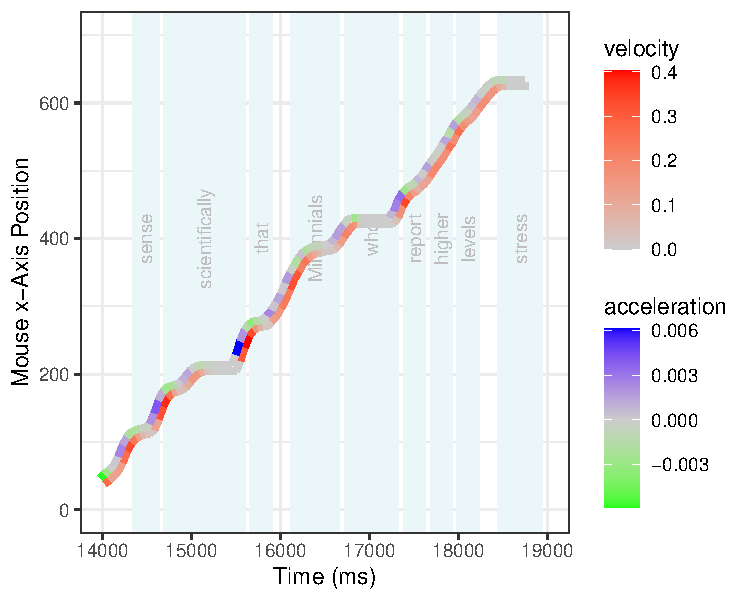
\includegraphics[width=0.46\textwidth]{images/reading_accel.pdf}
    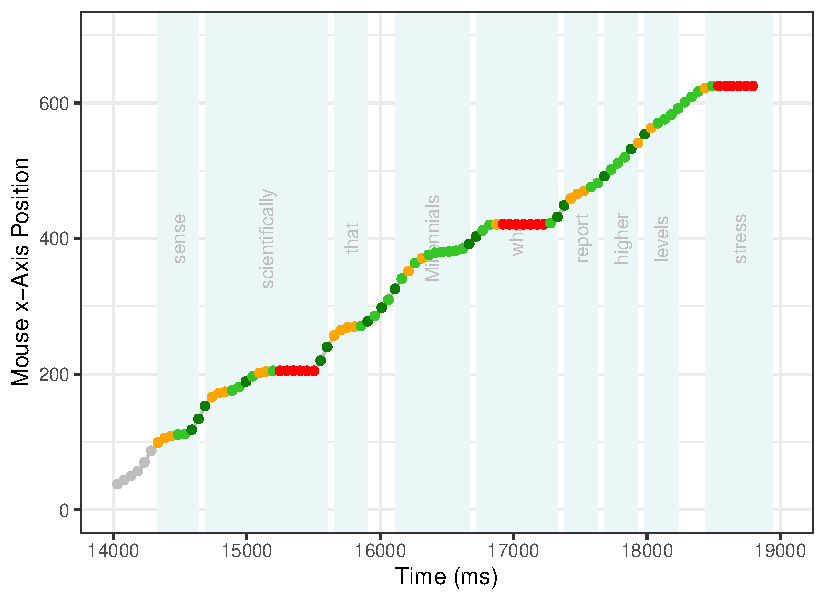
\includegraphics[width=0.50\textwidth]{images/reading_samples.pdf}
    \caption{\change{\textbf{\motr Reading Strategies:} The left panel shows the velocity (red) and acceleration (blue/green) for one participant reading a portion of the Provo corpus. The right panel shows the samples taken during this period, which are categorized into true fixations, decelerations, accelerations, movements of constant velocity, and offscreen time. Light blue background bands indicate associations with words, which are used to compute reading measures.}}
    \label{fig:basic-behavior}
\end{figure*}
\begin{figure*}[th!]
    \centering
    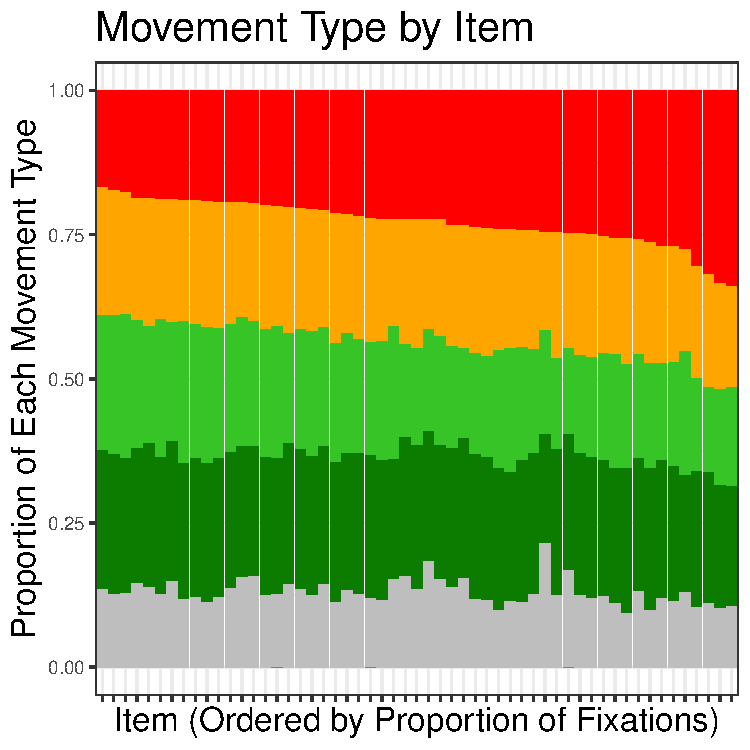
\includegraphics[width=0.27\textwidth]{images/item_movement.pdf}
    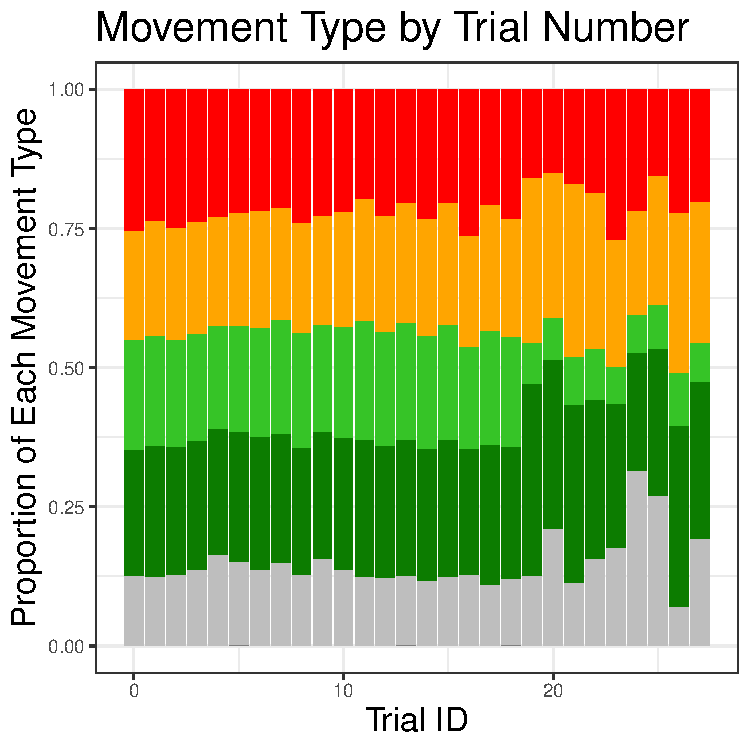
\includegraphics[width=0.27\textwidth]{images/trial_movement.pdf}
    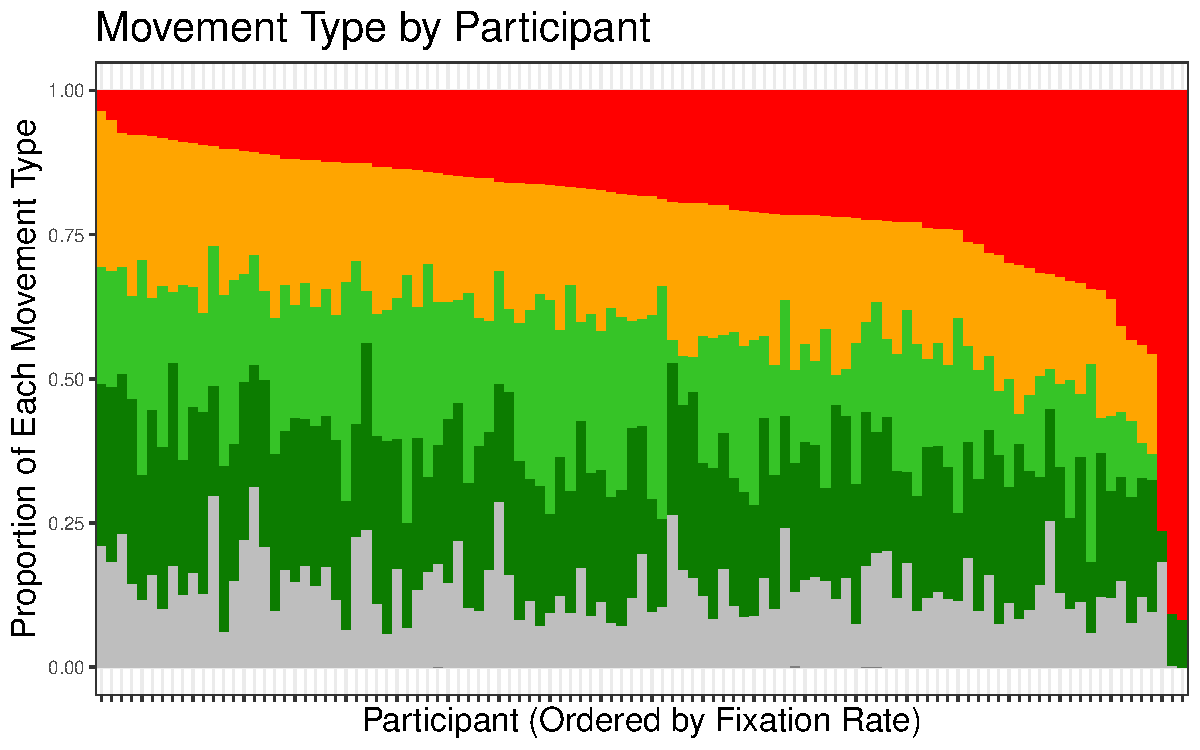
\includegraphics[width=0.43\textwidth]{images/participant_movement.pdf}
    \caption{\change{\textbf{Movement type by trial, item, and participant:} Bars show the proportion of samples from each movement type, categorized as true fixations (red), decelerations (orange), other types of movement (green), and offscreen time (gray).}}
    \label{fig:movement-types}
\end{figure*}

\change{How does the use of \motr change during an experiment, between items, and between participants? To visualize these differences, we plot the proportion of movement types broken down by various factors in Figure \ref{fig:movement-types}. On the left panel, we break movement type down by the different items (i.e., short paragraphs) in the Provo corpus, ordered by the proportion samples that were counted as true fixations. Although there is some variation, we observe roughly a similar proportion of fixations between items, ranging from $16$\% to $34$\%, with an average of $23$\%. Breaking down fixation by trial type (middle panel), again, we observe relative consistency throughout the experiment. %To test this, statistically, we fit a Bayesian logistic regression model to predict whether a given sample is a fixation or not, with a sole predictor of trial number, and random intercepts and slopes for item ID and participant ID\footnote{Our model call to \texttt{brms} was \texttt{is\_fixation $\sim$ trial\_id + (trial\_id | item\_id) + (trial\_id|subj\_id)}.} The model had two chains, each with $500$ warmup steps and $2,000$ samples. We find \textbf{... results ...}. 
Turning to the type of movement by participant (right panel), we find more variation. In particular, we observe a handful of participants whose behavior is similar to eye-tracking, and who produce primarily fixations and saccadic-like jerky movements with the mouse. That being said, the median participant is relatively well-balanced between the five types of movements. It is from this middle distribution that we drew the participant whose movements are visualized in Figure \ref{fig:basic-behavior}.}


\begin{figure*}[]
    \centering
    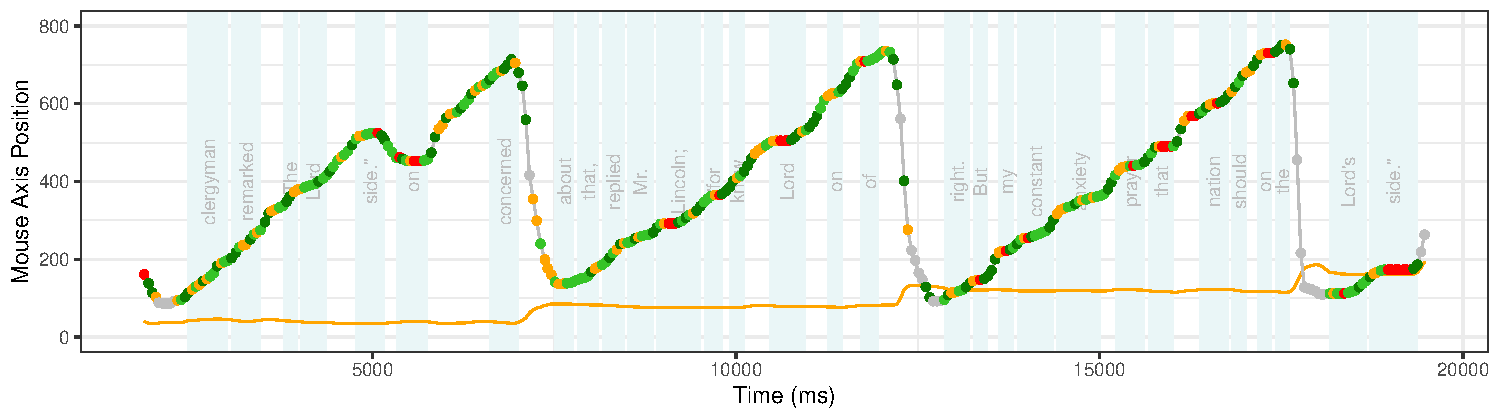
\includegraphics[width=0.99\textwidth]{images/reader_102_10.pdf}
    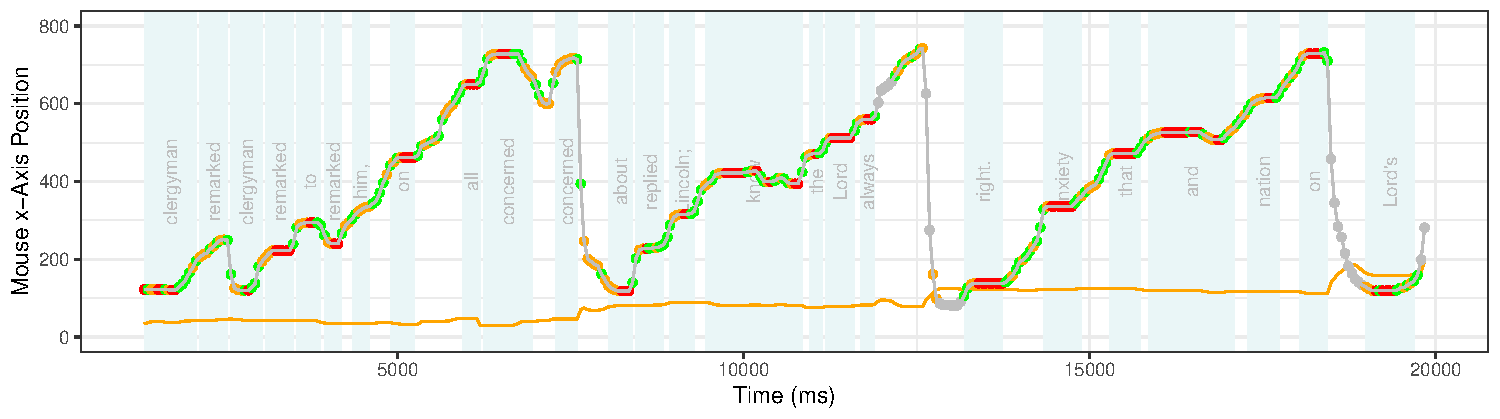
\includegraphics[width=0.99\textwidth]{images/reader_32_10.pdf}
    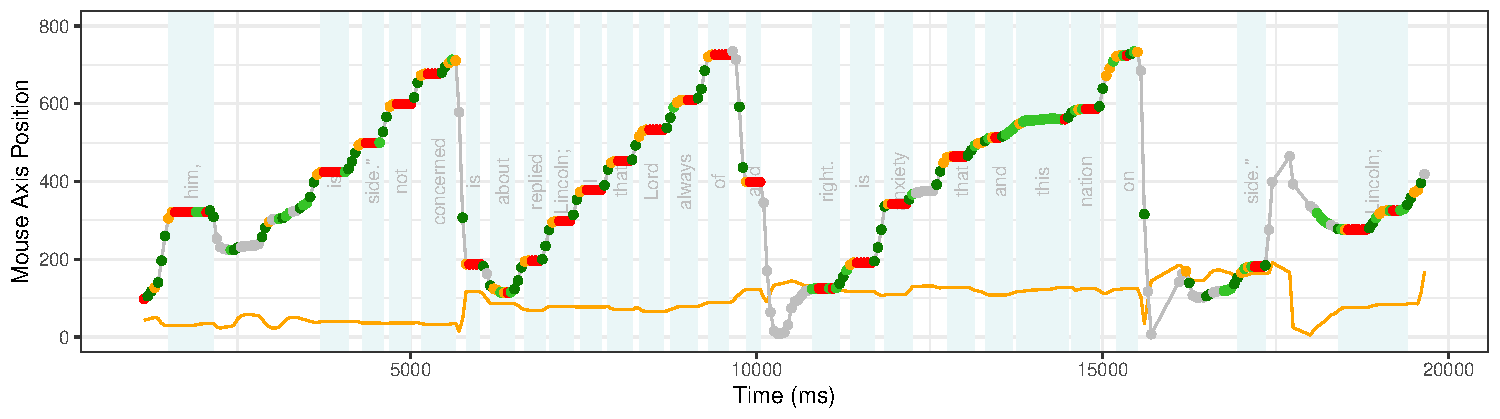
\includegraphics[width=0.99\textwidth]{images/reader_42_10.pdf}
    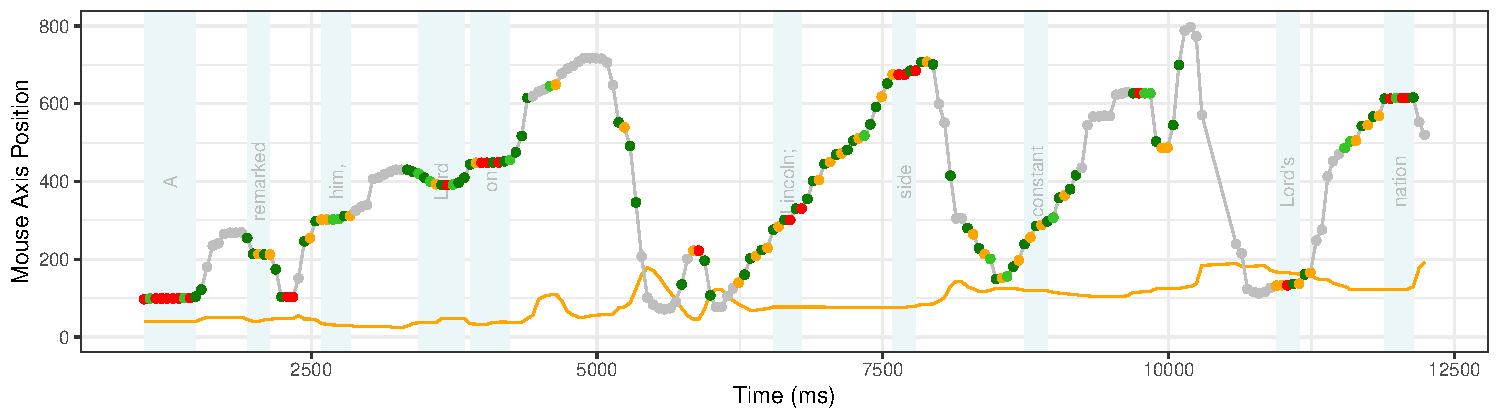
\includegraphics[width=0.99\textwidth]{images/reader_11_10.pdf}
    \caption{\small \change{\textbf{Examples of different reading strategies:} Smoother movements with no fixations (top row), fixation-based strategies (middle rows), and more random mouse movements (bottom row). In this case, the bottom-row trial would be filtered, as the participant associates with fewer than $20$\% of total words. The text is: \word{A clergyman remarked to him, ``The Lord is on our side.'' ``I am not at all concerned about that,'' replied Mr. Lincoln; ``for I know that the Lord is always on the side of the right. But it is my constant anxiety and prayer that I and this nation should be on the Lord's side.''}}}
    % Change axis labels so it's "mouse position in pixels" Add labels for line jumps and regressions. Add legend for x vs. y axis difference. And change the velocity/acceleration (movement type) coding. Change the legend for the movement type (in above figure as well).
    \label{fig:reading_examples}
\end{figure*}

\change{To give a better sense of the range of participant behavior, Figure \ref{fig:reading_examples} visualizes reading from four different participants whose use of \motr differs. In these figures, the sharp downward lines indicate times when participants move their mouse to the beginning of the next line of text. The blue bands indicate the associations, which are the result of our post-processing pipeline and contribute towards a word's reading time measures. Orange lines show the participant's $y$-axis location. The top row shows a participant who produces a smooth scan across the text, and who slows down, rather than fixating, at unexpected words, for example around \word{prayer} around 16000\,ms. The middle two rows show participants who produce more fixations. Finally, the bottom row shows a participant who is using the tool \emph{not} as intended, with lots of quick, seemingly random movements and offscreen time. In this case, this trial would be excluded during our data filtering step, as the participant associates with fewer than 20\% of the total words in the text.}


\subsection{Analysis 2: Comparing MoTR, Bidirectional SPR, and eye-tracking} \label{sec:correlations}

\change{For this analysis we compare \motr to BSPR by asking how well each measurement correlates with eye-tracking, as well as with word-level statistics.} For these analyses skipped words were handled in two ways, resulting in two different \motr datasets: \change{For the first dataset, which we will indicate with the tag \word{(w/ 0s)},} skipped words were given a reading time of zero and included in the computation of gaze duration and go past times. In the second dataset, \change{which has the tag \word{(drop 0s)},} skipped words were dropped from the analysis. \change{This was done to investigate the role of zeros in our post-processing pipeline, and how they affected the correlations between MoTR and eye-tracking data.} Generally, in reading time studies that look at differences in reading times between conditions words that are skipped on a first pass are simply dropped from the analysis. This is done, partly, to ensure that reading times for each word are roughly normally distributed around the mean reading time, which is a requirement for many statistical models. However, in this analysis, we are not interested in comparing the differences in reading times between conditions, but rather in the average reading times across many participants between different modalities. Excluding zeros from these cross-participant average reading times arguably discards important information about the amount of time some participants spent reading the word, which is 0 milliseconds if the word is skipped. This same data analysis choice has been done in a few recent studies (e.g., \citealp{pimentel2022effect} and \citealp{wilcox2023testing}). \change{However, as \word{drop 0s} is considered more standard, we will focus our discussion on the results of this analysis.}

For all analyses, only words that were fixated on during the first pass were included in the calculation of the first-pass regression probability. \change{Skipped words were not included in the computation of regression probabilities because landing on a word is a precondition for the decision to regress at that word.} As noted above, when looking at the relationship between \motr and eye-tracking, all analyses were run on cross-participant averages of reading times, as was done in the prior literature, e.g., \citet{smith2013effect, wilcox2020predictive} (although, cf. \citealp{hoover-etal-2021-linguistic}). \looseness=-1


\subsubsection{Correlation with eye-tracking Data} \label{sec:eyetracking-correlation}

\afterpage{
\begin{figure*}[ht]
    \centering
    \begin{minipage}{0.98\textwidth}
    \centering
    \small
    %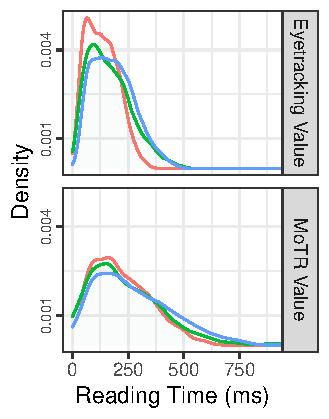
\includegraphics[width=0.23\textwidth]{images/density.pdf}
    % 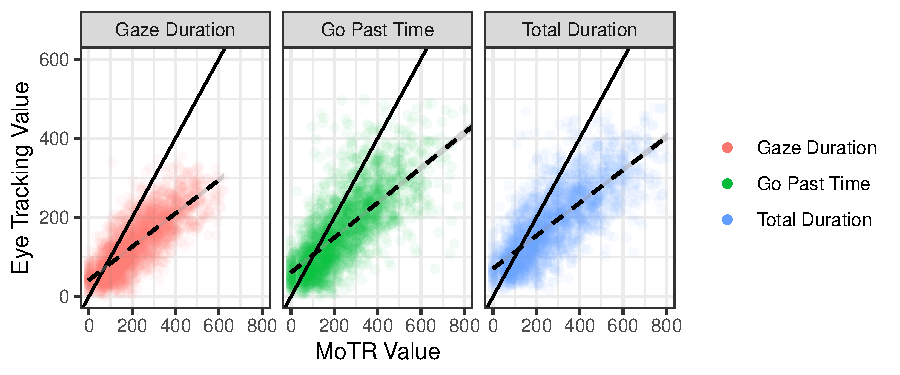
\includegraphics[width=0.73\textwidth]{images/metric_cor.pdf}
    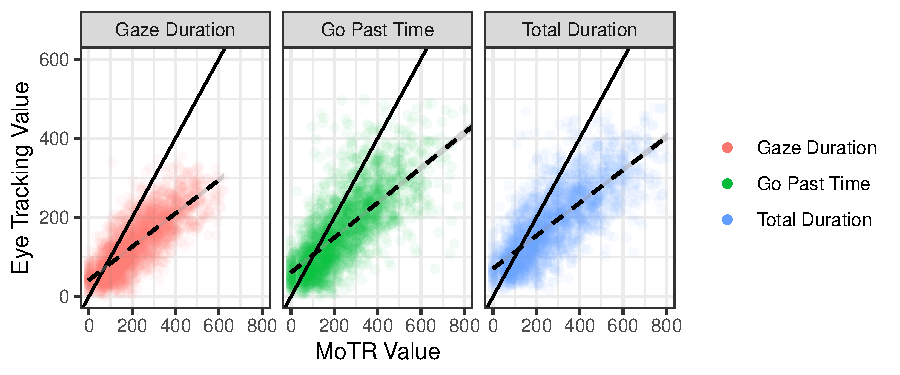
\includegraphics[width=0.95\textwidth]{images/metric_cor.pdf}
    \vspace{-0.3cm}
    \caption{ \small \textbf{Correlation Between \motr/BSPR and eye-tracking:} Data excludes RTs of zero (i.e., it is \emph{drop 0s}). The solid black line is the $x=y$ line. The dotted black line is the linear line of best fit.}
    % Add comparison between MoTR and BSPR
    \label{fig:motr_eyetr_comp}
    \end{minipage}
\end{figure*}
\begin{table}[ht]
    \small
    \centering
    \begin{tabular}{ c | c | c | c | c }
    \toprule
         & Gaze Duration & Go Past Time & Total Duration & Regression Prob.\footnotemark \\
    \midrule
        \makecell{\motr (w/ $0$s)} & \redcell{0.83 [0.82, 0.85]} & \redcell{0.78 [0.76, 0.80]} & \redcell{0.82 [0.81, 0.84]} & \redcell{0.16 [0.12, 0.19]} \\
        \makecell{\motr (drop $0$s)} & \greencell{0.51 [0.48, 0.54]} & \greencell{0.42 [0.39, 0.45]} & \greencell{0.62 [0.59, 0.65]} & \greencell{0.19 [0.14, 0.24]} \\
        \midrule
        \makecell{BSPR (w/ $0$s)} & \redcell{0.36 [0.32, 0.40]} & \redcell{0.29 [0.26, 0.34]} & \redcell{0.37 [0.33, 0.41]} & \redcell{-}\\
        \makecell{BSPR(drop $0$s)} & \greencell{0.35 [0.31, 0.39]} & \greencell{0.26 [0.22, 0.30]} & \greencell{0.40 [0.36, 0.44]} & \greencell{-}\\
        \midrule
        \makecell{Self Eye-Tr. (w/ $0$s)} & \redcell{0.93 [0.92, 0.93]} & \redcell{0.93 [0.92, 0.94]} & \redcell{0.93 [0.92, 0.93]} & \redcell{0.60 [0.57, 0.62]} \\
        \makecell{Self Eye-Tr. (drop $0$s)} & \greencell{0.75 [0.73, 0.78]} & \greencell{0.63 [0.60, 0.66]} & \greencell{0.81 [0.79, 0.82]} & \greencell{0.58 [0.55, 0.61]} \\
        % Add the "with self" to the caption!
        % To the caption add that we don't compute the correlations because there is too little data (say exactly how little data there is, and that the models didn't converge after x iterations.) Say in the text: "Although technically possible, people don't actually do these regressions." Add the skipping rate from BSPR and MoTR in the text, and say something similar.
    \bottomrule
    \end{tabular}
    \caption{\textbf{Correlation with eye-tracking:} Posterior means and 95\% CrIs. The top rows show the correlation over the whole dataset. Bottom two rows show the correlation between two splits of the eye-tracking dataset as an upper bound.}
    \label{tab:motr_eyetr_cor}
\end{table}
%\footnotetext{Using unranked, original data with the same \texttt{Stan} model yielded similar results. \change{MoTR (w/ 0s): 0.18 [0.14, 0.23]; MoTR (drop 0s): 0.21 [0.16, 0.27]; eye-tracking (w/ 0s): 0.67 [0.65, 0.70]; eye-tracking (drop 0s): 0.66 [0.63, 0.69].} \todo{Add data or explanation for BSPR}}
}


To compute correlations, we ran the Bayesian correlation analysis proposed in \cite{behseta2009bayesian}, which is more robust to outlier effects than standard Pearson correlations \citep{Matzke2017}. For each correlation, we report the posterior means and 95\% credible intervals for the correlation coefficient, $r$. For reading time correlations, we assume a bivariate $t$ distribution as the likelihood, which can be seen as a generalization of the bivariate normal distribution assumed by Pearson's correlation test. For regression probability, models achieved poor fit assuming the $t$ distribution. Thus, we report the results of a Spearman rank correlation test instead, which, unlike Pearson's correlation, is a non-parametric test without assuming a linear relationship between the variables, nor a normal distribution of the variables \citep{spearman1961proof}.

%For all the correlations, we assume a bivariate $t$ distribution as the likelihood, which can be seen as a generalization of the bivariate normal distribution with heavier tails allowing for more noises. An exception is made for the regression probability correlation between \texttt{motr} and eye-tracking. Since the original regression probabilities exhibit a "U" shaped distribution rather than normality, we ranked the data to achieve a more normal distribution. 
%Regularizing priors were assigned to the model parameters. For the RT models and the ranked FPReg probability correlation models, the priors for \(\mu\) and \(\sigma\) are \(\mu, \sigma \sim \mathcal{N}(150, 100)\), while \(\nu \sim \text{Gamma}(2, 0.1)\), and \(\rho \sim \text{Uniform}(-1, 1)\). In the eye-tracking self correlation regression model, the priors for \(\mu\) and \(\sigma\) are adjusted to \(\mu, \sigma \sim \mathcal{N}_{+}(0, 1)\) to reflect that the regression probabilities range between 0 and 1. We also adjusted the prior for scale parameters \(\sigma\) and mean parameters \(\mu\) to \(\sigma \sim \mathcal{N}(0, 100)\) to model correlation with word-level statistics according to our knowledge about these word-level properties. All the scale parameters \(\sigma\) follow \(\sigma \sim \mathcal{N}(0, 100)\) and the mean parameters \(\mu\) follow the same distribution, \(\mu \sim \mathcal{N}(0, 100)\). As in the first experiment, we used four chains  with 4000 iterations each, with the first 2000 for warming up. The convergence examinations are the same as for Experiment 1. We fit models using \texttt{Stan} \citep{carpenter2017stan}.

All the regression models had regularizing priors. For the RT models and the ranked FPReg probability correlation models, position parameter \(\mu\) followed a \(\mathcal{N}(150, 100)\) distribution and scale parameter \(\sigma\) followed a \(\mathcal{N}_{+}(150, 100)\) distribution.  The \(\mu\) prior suggested that the center of either \motr or eye-tracking data was likely within a range of 350. The wide \(\sigma\) prior reflected our uncertainty about the variability present in the two data sets. The \(\nu\) parameter, governing the degrees of freedom for the student t-distributions, was modeled with a \(\text{Gamma}(2, 0.1)\), making a wide range of values, from 0 to 80 to be very likely.
The \(\rho\) parameter was uninformative, following \( \text{Uniform}(-1, 1)\). As in the first experiment, we used four chains with 4000 iterations of which the first 2000 were warm-up. The convergence of the models was verified by examining the \(\hat{R}\)-statistic and trace plots \citep{gelman1995bayesian}. We fit models using \texttt{Stan} \citep{carpenter2017stan}. \change{Because of the extremely small number of regressions in the BSPR data---a regression 0.01 vs. 0.04 in \motr and 0.15 in eye-tracking---these models did not converge. Instead of reporting correlations from non-converged models we simply mark the correlations with a dash in tables.}

%Primarily, we're interested in the relationship between \motr data and eye-tracking data. We explore this relationship in two ways. First, we compare the distribution of reading times for each of the three metrics (gaze duration, go past time and total duration). These density plots can be seen in Figure~\ref{fig:motr_eyetr_comp}, left facet, with the eye-tracking data on top and the \motr data below. As expected, we find that gaze duration is slightly left-skewed compared to go past time and total duration for both measures, meaning that we find shorter reading times on average for this metric. Overall, we can see that the \motr data has a longer tail of reading times, with gaze durations, go past times and total durations that are longer than 500ms. These data verify that \motr is able to capture meaningful differences between the metrics, on aggregate, and that \motr reading times are slightly longer than eye-tracking reading times.

We visualize the relationship between \motr/BSPR and eye-tracking data in Figure \ref{fig:motr_eyetr_comp}. Here, the solid black line shows the $x=y$ line, and the dotted black line shows the linear line of best fit. \change{There are two things worth noting here: First, both the \motr and BSPR data seem, at least visually, to be linearly correlated with the eye-tracking data. Second, the \motr and BSPR data are rightward skewed,} meaning that their reading times tend to be slightly longer than eye-tracking reading times for the same word.

How well do the \motr and BSPR data correlate with the eye-tracking data? To compute an upper bound, we split the eye-tracking data into two groups, based on the participant ID assigned in the Provo dataset. Participants with ID less than 42 were assigned to the first group, while those with ID greater than 42 were assigned to the second. To compute an upper bound for correlation, we simply compute the correlation between the by-word average for each of the two groups. For this model, the priors for \(\mu\) and \(\sigma\) were narrowed to \(\mathcal{N}(0, 1)\) and \(\mathcal{N}_{+}(0, 1)\), respectively, due to the lower variability in the eye-tracking RTs. %To model correlation with word-level statistics, we also adjusted the \(\mu\) prior to be \(\mathcal{N}(0, 100)\) and \(\sigma\) to \(\mathcal{N}_{+}(0, 100)\). 
\change{We compute these correlations for both \word{drop 0s} and \word{w/ 0s} versions of the Provo dataset.}

The results can be seen in Table \ref{tab:motr_eyetr_cor}, with the \motr/eye-tracking correlation on the top rows, the BSPR/eye-tracking correlations in the middle rows, and the eye-tracking self correlations on the bottom. 
\change{There are four high-level trends that we would like to highlight: First, for every mouse-based metric (i.e., gaze duration, go past time, and total duration), \motr achieves higher correlations than BSPR. Second, despite its relatively robust correlations, both metrics are not as well correlated as eye-tracking is with itself. Third, correlations tend to be stronger when skipped words are included in the analysis (i.e., in the \word{w/ 0s} conditions), suggesting that treating skipped words as having an RT of zero produces \motr and BSPR data that is more comparable to eye-tracking data. Fourth, one place where we observe lower correlations is in first-pass regression probability}, where the correlation is 0.16 when including skips and 0.19 without skips. The self-regression probability correlation within eye-tracking is at 0.60 (w/ 0s) and 0.58 (drop 0s), which, while higher, is still lower than the self-correlation for the reading time measures.

%Overall, we find strong correlations for each of the reading time metrics when skipped words were included (top row), and weaker correlations when skipped words were dropped (middle row). This suggests that treating skipped words as having an RT of zero produces \motr data that is more comparable to eye-tracking data, meaning that this correlation is partially determined by our choice of $f_{min}$. %For the rest of the analyses presented in this section, we will use this skip-inclusive data.

%In order to get an absolute sense of how well \motr is capturing the eye-tracking data we can simply normalize the \motr correlation by the self eye-tracking correlation. When we do this, for the top row, we get a normalized score of $0.88$ for gaze duration, $0.86$ for go past time and $0.85$ for total duration, suggesting that \motr is similarly correlated for each of the metrics, but the best so for gaze duration.

%Interestingly, the one place where we do not observe strong correlations with eye-tracking is in first-pass regression probability, where the correlation is 0.16 when including skips and 0.17 without skips. The self-regression probability correlation within eye-tracking is at 0.63, which, while higher, is still lower than the self-regression correlation for the reading time measures. 

\change{One potential concern is that while \motr regression correlation is low, the correlation for go past time, which is largely determined by the presence or absence of regressions, is still relatively high. How can this be the case? In Table \ref{tab:motr_eyetr_cor} we find stronger correlations for gaze duration than for go past time, both for the drop 0s and w/ 0s analyses. Therefore, adding information about regressions decreases the correlation between eye-tracking and MoTR, which is in line with what we would expect. What this tells us is that the total number of regressions, both in eye-tracking and MoTR, is not large enough to impact the overall reasonably high correlation between the two metrics, when computed over a large dataset.}

We hypothesize that the lower regression correlation in \motr is due to the different amount of effort required to initiate a regression between the two paradigms. In eye-tracking, regressions (indeed, all saccades) are achieved by simply moving the gaze, however in \motr participants must plan an execution of a more complicated hand movement, which must be coordinated with a gaze movement as well. One effect of this is that it could raise the activation barrier for regressive saccades. \change{Framed in terms of trying to predict eye-tracking regressions from \motr regressions, the high activation cost of the latter could result in a low number of \emph{false positives}, but a high number of \emph{false negatives}. That is, when a word triggers a regression in \motr the same word is likely to trigger a regression in eye-tracking, but only a subset of the words that trigger eye-tracking regressions also trigger \motr regressions.} To test this hypothesis, we look at the distribution of regression-triggering words under each metric. Words were counted as regression-triggering words if any participant initiated a regression from it during its first pass. We found that $98\%$ of regression-triggering words in \motr were also regression-triggering in eye-tracking, however, only $38\%$ of regression-triggering words from eye-tracking also triggered a regression in \motr. This confirmed our hypothesis, that \motr is good at picking up eye-tracking regressions with high precision, but only picks up a subset of the regressions that can be found in eye-tracking.


\begin{figure}[]
    \centering
    \begin{minipage}{\textwidth}
    \centering
    \small
    % 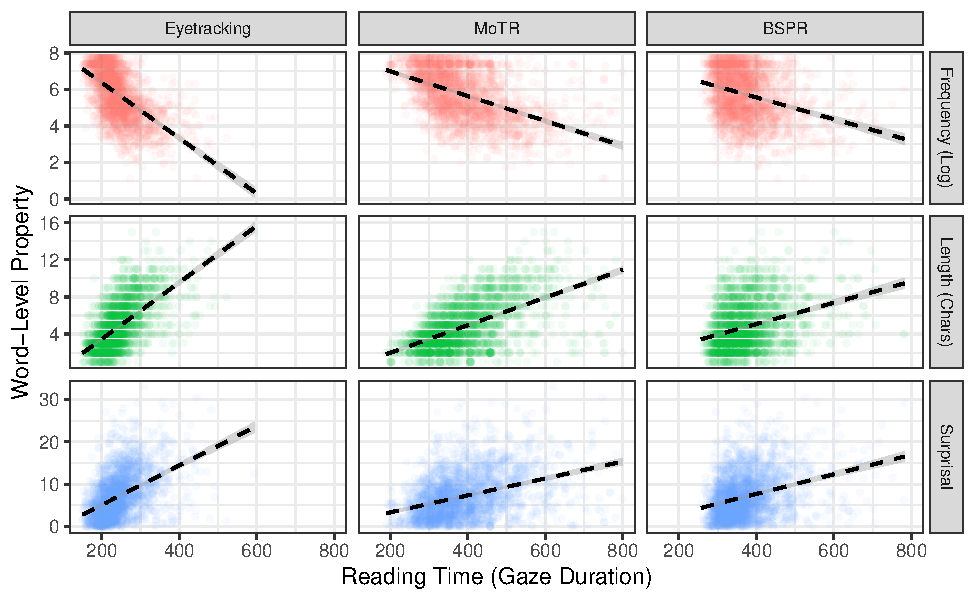
\includegraphics[width=\textwidth]{images/word_prop_comps.pdf}
    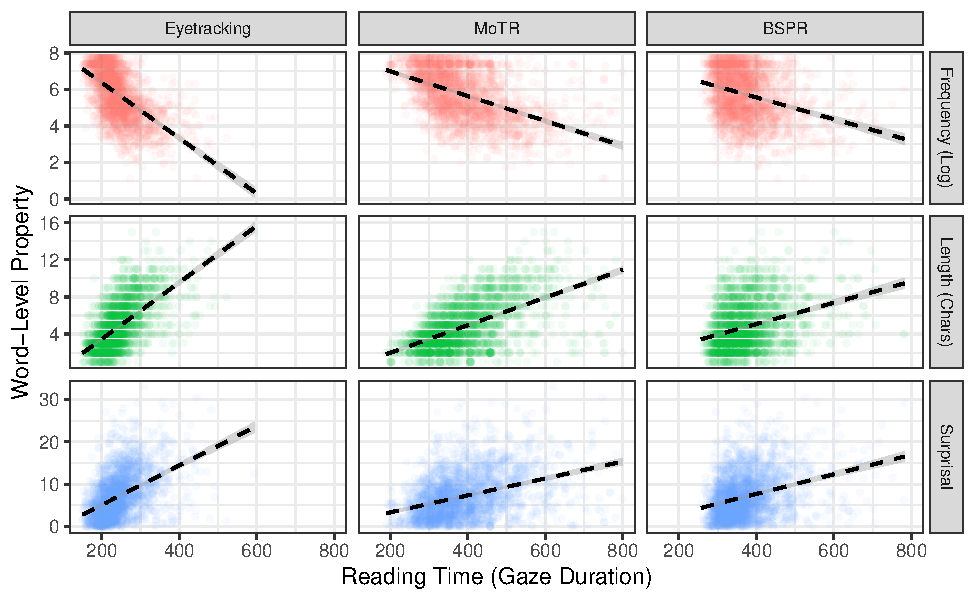
\includegraphics[width=\textwidth]{images/word_prop_comps.pdf}
    \vspace{-0.8cm}
    \caption{ \small \textbf{Comparison Between \motr, Eyetracking, and Various Word-Level Statistics:} Results are for Gaze Duration, and do not include skipped words (i.e., data is \emph{drop 0s}).}
    % ADD in the bayesian regression lines instead of these linear lines of best fit
    % Also change the axis labels
    \label{fig:word-comp}
    \end{minipage}
    \vspace{0.5cm}
    \begin{tabular}{ c | c | c | c }
    \toprule
         & Log Frequency & Length & Surprisal \\
    \midrule
        \motr (w/ $0$s) & \redcell{-0.77 [-0.79, -0.76]} & \redcell{0.90 [0.89, 0.91]} & \redcell{0.54 [0.51, 0.57]} \\
        \motr (drop $0$s) & \greencell{-0.58 [-0.60, -0.55]} & \greencell{0.68 [0.66, 0.70]} & \greencell{0.43 [0.40, 0.47]} \\
        \midrule
        BSPR (w/ $0$s) & \redcell{-0.29 [-0.33, -0.25]} & \redcell{0.30 [0.26, 0.34]} & \redcell{0.31 [0.27, 0.35]} \\
        BSPR (drop $0$s) & \greencell{-0.30 [-0.34, -0.26]} & \greencell{0.31 [0.27, 0.35]} & \greencell{0.32 [0.28, 0.36]} \\
        \midrule
        Eye-Tr. (w/ $0$s) & \redcell{-0.82 [-0.83, -0.80]} & \redcell{0.88 [0.87, 0.89]} & \redcell{0.60 [0.57, 0.63]} \\
        Eye-Tr. (drop $0$s) & \greencell{-0.60 [-0.63, -0.57]} & \greencell{0.64 [0.61, 0.66]} & \greencell{0.51 [0.48, 0.54]} \\
    \bottomrule
    \end{tabular}
    \captionof{table}{\textbf{Correlation with word-level statistics:} We report the posterior means and 95\% credible intervals of the correlation coefficient of our Bayesian model.}
    \label{tab:stat_cors}
\end{figure}

\subsubsection{Relationship to Word-Level Statistics}

We investigate the relationship between \motr, BSPR eye-tracking, and various word-level statistical properties that have been shown to impact reading times in naturalistic settings. Our word-level properties are log frequency, as reported in \citet{speer2022wordfreq}; word length in characters, and \defn{surprisal}. Surprisal is the negative log probably of a word, given its context, i.e., $s(w_t) = - \log p(w_t \mid \mathbf{w_{<t}})$, and is known to be a strong predictor of reading time above and beyond length and frequency \citep{hale2001probabilistic, levy2008expectation, smith2013effect, wilcox2020predictive, wilcox2023testing}. Here we look simply at the correlation, however, we conduct a more in-depth investigation into the functional relationship between surprisal and \motr data in the next section. All of our surprisal values are estimated from GPT-2 \citep{radford2019language}, a large language model that has been trained to predict the distribution over sub-word units (called \word{tokens}) given their context. To turn predictions over tokens into predictions over words we simply sum the surprisal over within-word tokens, following the chain rule of probabilities. For this analysis, correlations are computed using the same methods as described in the previous section, however here we adjusted the \(\mu\) prior to \(\mathcal{N}(0, 100)\) and \(\sigma\) to \(\mathcal{N}_{+}(0, 100)\). 

Figure \ref{fig:word-comp} shows the relationship between eye-tracking (left column), \motr values (middle column), and BSPR values (right column), against our various word-level properties along the different rows. \change{Data is plotted from the drop $0$s version of the dataset.} As the results are similar across the different metrics, we show only data for gaze duration. Correlations are reported in Table \ref{tab:stat_cors}. \change{We find similar trends as before: First, \motr correlations are higher than BSPR correlations, although they are slightly lower than the correlations found for eye-tracking. Second, there tend to be slightly stronger correlations for the w/ 0 datasets compared to the drop 0 datasets. Overall, we find that log frequency and length are more highly correlated with \motr than surprisal. In the next section, we follow up on this observation and take a deeper look at the relationship between surprisal and \motr reading times. }


\subsection{The Functional Relationship Between \motr and Surprisal} \label{sec:info-theory}

In this section, we investigate the functional relationship between \motr RTs \change{and surprisal}. Following \citet{smith2013effect} and \citet{wilcox2020predictive}, we produce a visualization of the relationship that can be inspected to determine if it is (roughly) linear. To do so, we use generalized additive models (GAMs), which are a class of models that can fit non-linear relationships between predictor variables and response variables. Given that the GAM has a less constrained hypothesis space than a linear model, if it finds a relationship that looks roughly linear, this is good evidence that the underlying effect is, itself, linear. \change{In addition, following more recent work \citep{hoover-etal-2021-linguistic, meister-etal-2021-revisiting, shain2022large, wilcox2023testing}, we complement these visualizations with statistical analyses that test for evidence for non-linearities in the relationship. To do so, we fit GAMs that enforce a linear relationship between surprisal and \motr RTs. We then use leave-one-out cross-validation to assess whether these linear GAMs are worse at predicting held-out data than the non-linear GAMs. If we do not find a difference in predictive power between these classes of models, this suggests that a linear surprisal--RT linking function is best characterized as linear.} 

To conduct these analyses we fit GAMs to predict the reading time of a word $w_t$ from its log frequency, length in characters, and surprisal as well as the log frequency, length, and surprisal of the previous word $w_{t-1}$. This was done due to the previous spillover effects which have been found for eye-tracking. As before, our frequencies are from \citet{speer2022wordfreq}, length is measured in the number of characters, and surprisal estimates are from GPT-2. In the GAM model, we include smooth terms for our surprisal values as well as tensor product terms for a non-linear interaction between log frequency and word length. GAMs are fit using the \texttt{mgcv} package in \texttt{R}.\footnote{A sample GAM call: \texttt{rt $\sim$ s(surp(w$_t$), bs = `cr', k = 6) + s(surp(w$_{t-1}$), bs = `cr', k = 6) + t\change{2}(freq(w$_t$), len(w$_t$), bs = `cr') + t\change{2}(freq(w$_{t-1}$), len(w$_{t-1}$), bs = `cr')}} To capture non-linearities in this model we set up a non-linear spline-based smooth for the effect of surprisal, which is restricted to six basis functions. The linear models are the same, except they include only linear terms for surprisal, instead of spline-based smooth terms.
We train models on twenty different folds of data. %%\footnote{Details about the fitting procedure are as follows: We specify that the RTs follow a Gamma distribution and use a log linking function. For the intercept, a normal distribution with mean \(6\) and standard deviation \(1\) was used. The reason for choosing this prior was the same as in Experiment 1. The fixed effects followed a normal distribution prior as \(b \sim \mathcal{N}(0, 0.5)\) which reflected our uncertainty about the effects our predictors have to the RTs and allows for significant effect for the predictors, while the smooth terms follow a Cauchy distribution with location \(0\) and scale \(0.5\), expressed as \(sds \sim \text{{Cauchy}}(0, 0.5)\). Lastly, the shape parameter is modeled with an exponential distribution with a rate of \(2\), expressed as \(\text{{shape}} \sim \text{{Exponential}}(2)\). We use four chains each with 4000 iterations, of which the first 2000 are warm-up. To ensure convergence, the fitting process is controlled with an adapt\_delta parameter of 0.99.} 
For fitting \change{the GAM model in a Bayesian framework}, we assumed RTs follow a Gamma distribution with a log link function.%\footnote{While Lognormal models with the same set of priors from Experiment 1 yielded similar outcomes, Gamma models better fit the data based on the posterior summary statistics and are therefore reported.} 
The intercept was set to a normal distribution \( \mathcal{N}(6, 1)\). The fixed effects were assigned a normal distribution prior \(b \sim \mathcal{N}(0, 0.5)\), reflecting our uncertainty about the predictors' impact on RTs and allowing for potentially large effect sizes. For the same reason, the smooth terms followed a Cauchy distribution, \(sds \sim \text{{Cauchy}}(0, 0.5)\), which was similar to normal distribution but with heavier tails, making it more tolerant of extreme values and less informative. The shape parameter followed an \(\text{{Exponential}}(2)\) distribution, providing flexibility while assuming an extremely long-tailed RT distribution to be unlikely. We used four chains each with 4000 iterations, of which the first 2000 were warm-ups. To ensure convergence, the fitting process is controlled with an \texttt{adapt\_delta} parameter of 0.99.

To produce visualizations, we sample the models' predicted reading times based on the surprisal of $w_t$ and $w_{t-1}$ for values from 0-20 in increments of 0.1. These samples thus give us the models' predicted slowdown due to surprisal across a wide range of surprisal values. We can inspect if the predicted slowdown due to surprisal grows linearly as a function of surprisal itself. Samples from our twenty different models were used to compute 95\% bootstrapped confidence intervals.

\begin{figure*}[t]
    \centering
    \begin{minipage}{0.98\textwidth}
    \centering
    \small
    % 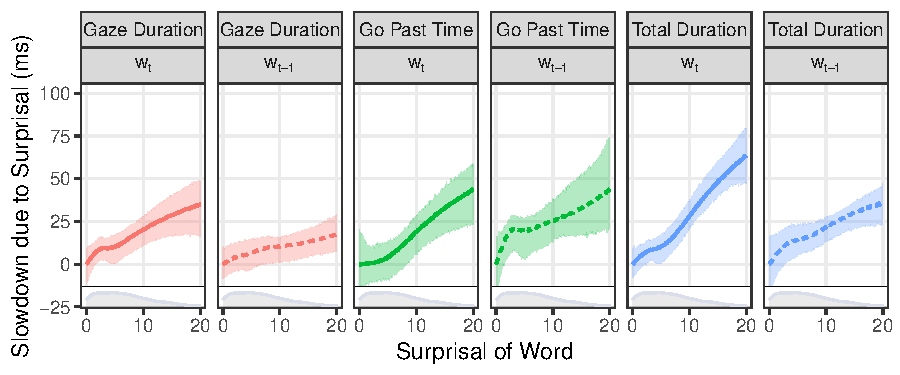
\includegraphics[width=\textwidth]{images/surp_rt_wt.pdf}
    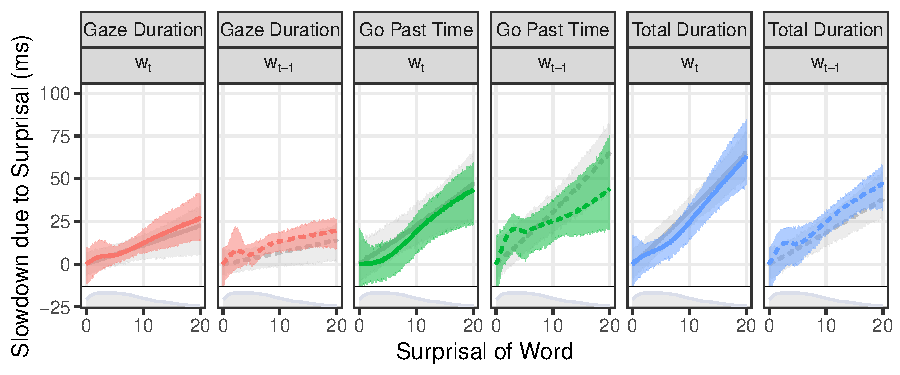
\includegraphics[width=\textwidth]{images/surp_rt_wt_combo.pdf}
    \vspace{-0.3cm}
    \caption{ \small \textbf{Relationship between surprisal and \motr reading times:} Shaded regions are bootstrapped 95\% confidence intervals. Solid lines indicate the slowdown due to the surprisal of the current word, $w_t$, whereas dotted lines indicate the slowdown due to surprisal of the previous word $w_{t-1}$. \change{Grey sub-plots in the background is the relationship fitted by GAMs that enforce a linear relationship between surprisal and MoTR RTs.} Grey sub-plots at the bottom show the distribution of surprisal in the corpus. }
    \label{fig:surp_motr_link}
    \end{minipage}
\end{figure*}


\todo{Add an explanation for the grey sub-plots of the linear GAMs?}The result of this procedure can be seen in Figure \ref{fig:surp_motr_link}, with different colors showing the different metrics. Slowdowns due to surprisal of the current word $w_t$ are shown with solid lines, whereas slowdowns due to the surprisal of the previous word $w_{t-1}$ are shown with dotted lines. We wish to draw out two points: First, we find a roughly linear relationship between surprisal and \motr RTs. The second point is that effects for surprisal for $w_t$ seem to be about as large as those for $w_{t-1}$. This is different from what has been observed for strongly incremental processing measurements such as the maze task, where the effect of surprisal of the previous word is essentially non-existent \citep{boyce2020stories}. However, it is in line with previous results for eye-tracking, where the effect of surprisal is about equivalent for $w_t$ and $w_{t-1}$ \citep{smith2013effect}.
% however go past times do appear to have a less directly linear relationship in the 0-5 surprisal range. This could be due to the fact that some low surprisal words initiate regressions, causing longer go past reading times than would be expected based on their surprisal. These same words are, however, not the target of subsequent regressions, which is why such non-linearities are not observed in the total duration data. 
%The second point is that effects of surprisal for $w_t$ tend to be larger than for $w_{t-1}$. For example, for gaze duration, a surprisal of 20 on $w_t$ is predicted to cause a slowdown of about 35 ms, a surprisal of 20 on $w_{t-1}$ is predicted to cause a slowdown of only about 25 ms. Interestingly, these results are in between patterns observed in eye-tracking data, where the effect of surprisal is about as strong for the current and previous word \citep{smith2013effect}, and other incremental processing techniques such as maze, where the effect of surprisal on the previous word has been found to be essentially non-existent \citep{boyce2020stories}.


\change{To test, statistically, whether there is evidence for a non-linear relationship between surprisal and \motr RTs, we conduct a model comparison between our linear and non-linear GAMs for each of our reading measures. We used leave-one-out cross-validation to compare the predictive accuracy between the two types of models, which involves testing each model on a single observation while training it on the remainder of the dataset \citep{vehtari2015efficient, vehtari2017practical}. This procedure produces a difference in log pointwise predictive density ($\Delta$ ELPD), where a negative value indicates higher predictive accuracy for the linear model. The findings align with the visual observations. First, for all models, the Pareto k diagnostic values are below 0.5, confirming that our leave-one-out estimates are reliable \citep{vehtari2015efficient}. Second, we observe a consistently negative, albeit modest, $\Delta$ ELPD, regardless of the reading time measurement used. For gaze duration the $\Delta$ ELPD is $-1.7$ with a standard error of $0.9$; for go past time it s $-1.4$ (SE: $1.4$); for total duration it is $-1.4$ (SE: $1.2$). These results indicate that, despite the increased parameter count of the non-linear models, the linear models are actually \emph{better} at predicting \motr reading times. This is likely because the non-linear models are overfitting to their training data. Overall, these data suggest that \motr reading times do preserve the linear functional relationship found in eye-tracking between processing times and surprisal.}


\section{Experiment 2: Attachment Preferences in English} \label{sec:exp1}

In this experiment, we ask whether \motr can measure well-studied processing patterns that have to do with attachment preference in English. Decades of psycholinguistic research has revealed that language processing is incremental, meaning that the processor builds syntactic representations on the fly and attempts to incorporate new material into the representation as soon as it is encountered. Often, the grammar constrains how new syntactic material can be added to the incremental representations. However, sometimes the new material is syntactically ambiguous, insofar as it can be grammatically incorporated into the syntactic parse at multiple different locations.

When this is the case, where do people choose to incorporate the material? \cite{frazier1979comprehending} argues that native speakers of English often show a preference for incorporating the material into the phrase that is currently being processed (referred to as the \defn{late closure} principle). This results in a processing strategy that favors lower attachment sites, i.e., ones that are further away from the root of the syntactic tree. \change{However, subsequent experiments have demonstrated that the late closure principle is not operative in other languages (e.g., Spanish, \citealp{cuetos1988cross}), or even a general preference in English \citep{gilboy1995argument}, and that other factors may influence attachment, such as modifying clause length \citep{hemforth2015relative} as well expectations about discourse \citep{rohde2011anticipating}. Despite this variability,} preference for low attachment in English has become something of a testing ground for new incremental processing measures, having previously been used to study the difference between maze, SPR, and eye-tracking \citep{witzel2012maze}, as well as between A-maze, L-maze, G-maze and self-paced reading \citep{boyce2020amaze}. In this section, we use the same materials as those originally presented in \cite{witzel2012maze} (and also used by \citealp{boyce2020amaze}) to compare \motr with these previous measurement tools.

\subsection{Materials and Methods}

\subsubsection{Materials}

% Macro for underline color
\setulcolor{CadetBlue}

We test three different types of attachment preferences. Following \cite{witzel2012maze} all of our materials are split into sentence regions, which are indicated with underlines in the examples below. Each sentence contains a pre-critical region, a critical region which is bolded in the examples below, and where we expect the strongest differences between conditions, as well as two post-critical regions, where we expect weaker effects. Region delineation is reconstructed from the examples given in Tables 1-6 of \cite{witzel2012maze}. In the next paragraphs, we walk through the materials for each of the three sub-experiments.

\paragraph{Adverb Attachment:} The first set of materials investigates the attachment of temporal adverbs, with the two conditions given in Example \ref{ex:adverb}, below. Both conditions include a matrix clause with a verb (here, the past-tense \word{wrote}) as well as a relative clause with a verb whose tense is mismatched to the main clause verb (here, the future tense \word{will deliver}). This is followed by an adverb whose temporal properties either match the relative clause or the matrix clause and force either a low attachment or high attachment reading. If low attachment is easier to process, then subjects should read this critical region more quickly when it agrees temporally with the relative clause, as opposed to the matrix clause.

\ex. Adverb Attachment \label{ex:adverb}
\a. \ul{Dan wrote the speech he will deliver} \ul{\textbf{next month}}, \ul{but he hasn't} \ul{practiced it yet.} ({\sc Low Attachment})
\b. \ul{Dan wrote the speech he will deliver} \ul{\textbf{last month}}, \ul{but he hasn't} \ul{practice it yet}. ({\sc High Attachment})

\paragraph{Coordination Clause Attachment \change{(NP/S Gardenpath)}:} The second set of materials test attachment preferences for coordination phrases, with conditions given in Example~\ref{ex:coordination}. Both conditions start with a transitive sentence and continue with a coordination phrase (\word{and the actor\dots} in the example below). In the \nocomma condition, the phrase can plausibly be coordinated with the object of the transitive verb to form a larger constituent (i.e., \word{the actress and the actor}), however this structural interpretation is later ruled out by the presence of a later verb (\word{quit}, in the example below). If the reader has committed to this locally plausible but globally implausible parse, they should find the disambiguating verb unexpected, and we would expect relatively longer reading times on it in this condition. In the \comma condition, a comma is inserted before the coordination phrase. In written text, commas can serve as cues to clause boundaries, rendering the coordination phrase unambiguously high-attached. This type of structural ambiguity is also known as an \change{\defn{NP/S Gardenpath}}.

\ex. NP vs. S (Coordination) Attachment \label{ex:coordination}
\a.  \ul{The producer replaced the actress, and the actor} \ul{\textbf{quit}} \ul{the movie} \ul{after the fight.} ({\sc Comma})
\b. \ul{The producer replaced the actress and the actor} \ul{\textbf{quit}} \ul{the movie} \ul{after the fight.} ({\sc No-comma})

\paragraph{Relative Clause Attachment:} The final set of materials tests preferences for relative clause attachment, with both conditions given in Example \ref{ex:relative_clause}. Here, sentences start with a Noun Phrase that has an attached Prepositional Phrase. Both NP and PP contain a grammatically gendered animate noun, for example, \word{brother} and \word{ballerina} in \ref{ex:relative_clause}. The sentence continues with a relative clause that includes a gendered reflexive pronoun. The pronoun either agrees with the gender of the second noun or the first noun, forcing either high or low attachment for the whole relative clause. If participants are expecting low attachment, we should find faster reading times when the reflexive pronoun matches the second noun and the RC can be attached low.

\ex. Relative Clause Attachment \label{ex:relative_clause}
\a. \ul{The brother of the ballerina who found} \ul{\textbf{herself}} \ul{in a lot of trouble} \ul{phoned home} ({\sc Low Attachment})
\b. \ul{The brother of the ballerina who found} \ul{\textbf{himself}} \ul{in a lot of trouble} \ul{phoned home} {\sc (High Attachment)}


\subsubsection{Methods}

Participants were shown the same instruction screen as described in Section \ref{sec:exp2} and were acclimatized to \motr with three practice trials before moving on to the main experiment. Our materials were the same as those used in \cite{witzel2012maze} and \cite{boyce2020amaze}. They include 48 items for each attachment type, balanced between conditions, as well as twenty-four filler sentences. Comprehension questions were all binary yes/no questions, balanced equally between \word{yes} and \word{no} correct responses. Half of the comprehension questions were written for the original \cite{witzel2012maze} paper, while the other half were created later by \cite{boyce2020amaze}. Questions from both batches follow the same format. 
%Items were presented according to a Latin Square to ensure that each participant did not read the same item under different conditions and that the participant was exposed to each condition the same number of times. 
Items were different between the conditions but balanced so that participants saw each condition the same number of times. The font size was chosen so that materials would fit on a single line when tested on a 13-inch monitor.

The experiment was run using Magpie and hosted on GitHub Pages. Our back end was implemented using Heroku. We recruited %197 
246 participants from Prolific\footnote{\url{https://www.prolific.co/}}. Participants were all native speakers of English, with IP addresses originating from within the United States. Participants were required to be using a desktop computer. While we cannot guarantee this, the choice of desktop was made so that participants would likely use a mouse and not a trackpad. Due to the large number of items in the experiment, we broke it into three sub-experiments with 59 items each, which took 14 minutes to complete, on average. Subjects were paid for their time and could not participate in more than one sub-experiment.


\subsubsection{Data Analysis}

%\begin{itemize}
    %\item Participants were filtered if we talked to them and they sounded like bots. Can we explain this further?
%\end{itemize}

As in the first experiment, we used three criteria to discard participant data: First, data from a given participant was completely discarded if the participant got fewer than 80\% of the comprehension questions correct. This threshold was chosen because it was the one used in \citet{boyce2020amaze}. Ten participants were excluded for this reason. Additionally, data from individual trials was excluded if the participant fixated on fewer than 20\% of the total words in the sentence, indicating that they were simply skimming. Skimming is a type of reading strategy where readers aim to understand the gist of a text, rather than its full semantic content. It is associated with more word skipping and longer saccades \citep{liao2021using}. A total of $9,075$ words (also about $\approx 1.5\%$ of the total data) were excluded for this reason. Words that were skipped during the first pass were not included in the computation of gaze durations and go past times. \change{Finally, RTs were excluded if they were below $f_{min}$ or above $f_{max}$, as described in Section \ref{sec:motr}}. \looseness=-1

For visualizations, we calculated the mean cross-participant per-word reading time for each sentence region and plotted the difference in means between conditions across items. For statistical tests, we fit a Bayesian mixed-effects model to the mean within-region per-word reading time separately for each measure, or the mean FPReg probability for each sentence region.
The models included the experimental condition (\highattach vs. \lowattach or \comma vs. \nocomma) as the sole fixed effect coded with sum contrasts (with \highattach being coded as 0.5 and \lowattach as -0.5), as well as by-item and by-subject random effects to capture the variability associated with both subjects and items and the correlation between the random effects. For our continuous reading measures (gaze duration, go past time, and total duration), we assumed a log-normal likelihood. For regressions, \change{which were binary variables (i.e., whether or not the participant regressed),} we used a Bernoulli distribution, and the relationship between the predictors and the response was modeled using a logit link function.

We used weakly informative priors in all our models to to integrate \change{domain expertise on RTs and regression probabilities from related real-time processing methodologies (e.g., eye-tracking),} while also accommodating methodological differences. For models predicting continuous measures (i.e., RTs), the intercept was set to follow a normal distribution \(\mathcal{N}(6, 1)\), translating to an expected grand mean RTs of $exp(6) \approx $ 403 ms and a 95\% RTs range of  $exp(4) \approx $ 54 ms to $exp(8) \approx $ 2980 ms. The slope's prior was configured to follow a normal distribution \(\mathcal{N}(0, 0.1)\), and variance components were modeled with \change{\(\text{{Exponential}}(2)\) to speed up sampling \citep{mcelreath2018statistical}}. These choices were informed by 
\citet{schad2021toward} and \citet{nicenboim2021introduction}, who analyzed related reading studies (i.e., \citealp{nicenboim2016high, vasishth2018statistical}) and our anticipation that the variability and differences in RTs across conditions would not be dramatic (i.e., over 800 ms). For the correlation matrix within the random effects variance-covariance structure, an LKJ prior was used with a shape parameter \(\nu = 2\) to reduce the influence of extreme correlations of ±1.

In the FPReg models, the intercept prior was \(\mathcal{N}(0, 2)\), signifying the unbiased starting point expectation in log-odds space. This translated to a baseline probability of 0.5 for initiating a regression, indicating no strong prior assumption either way. The slope and the variance components followed \(\mathcal{N}(0, 1)\) \change{and \(\mathcal{N}_+(0, 1)\) priors, respectively}, implying that we do not have a prior belief that different conditions or random effects will drastically increase or decrease the regression probability. We used the same LKJ prior as for the continuous dependent variables. These choices were inspired by and aligned with \citet{mertzen2023syntactic}.

Each model ran on four chains with 4000 iterations; the first 2000 served as warm-up and were excluded from inference. The convergence of the models was verified by examining the \(\hat{R}\)-statistic and trace plots \citep{gelman1995bayesian}. Reading time effects are reported in milliseconds, having been transformed back from the log-scale \citep{nicenboim2021introduction}.
%on the log-transformed mean per-word reading time for each sentence region with a maximal effects structure (i.e., by-subject and by-item random slopes and intercepts). We include the experimental condition (\textsc{high attachment} vs. \textsc{low attachment} or \textsc{comma} vs. \textsc{no-comma}) as the sole fixed effect, which we code with 1/0 dummy coding.
In the text, we report the mean and 95\% credible intervals (CrIs)  for the model's posterior distribution of the effect of the experimental condition. If the 95\% CrIs do not cross zero, we take this as good evidence for an effect of condition on participants' reading times.
%and report its $p$-value. 
%For our reading time measures---gaze duration, go past time and total duration---we report the result of a Bayesian linear mixed effects model, fit on log-transformed data. For first-pass regression probability we report the result from a Bayesian logistic mixed effects models. 
All models were fit using the \texttt{brms} package \citep{burkner2017brms} in \texttt{R}, which fits models using \texttt{Stan} \citep{carpenter2017stan}.


\subsection{Results}

\subsubsection{Main Results}

\newcommand{\stats}[3]{$\beta=$#1 [#2, #3]\xspace}


The results of our Bayesian models can be seen in Figure \ref{fig:modeling-results}, which shows the posterior mean and 95\% credible intervals for the sole fixed effect of condition in our model. Although this figure shows modeling results for multiple measurements (\motr, SPR, and maze), we will focus on \motr results here and discuss the comparison between measurements in the next section. In addition to these modeling results, Figure \ref{fig:target-results} shows the means of the raw RT data. To give a sense of the comparison between \motr and eye-tracking, we plot the eye-tracking differences between the condition/region averages reported in \citet{witzel2012maze} in \textcolor{teal}{teal} alongside our own data.


\begin{figure*}[t]
    \centering
    \begin{minipage}{\textwidth}
    \centering
    \small
    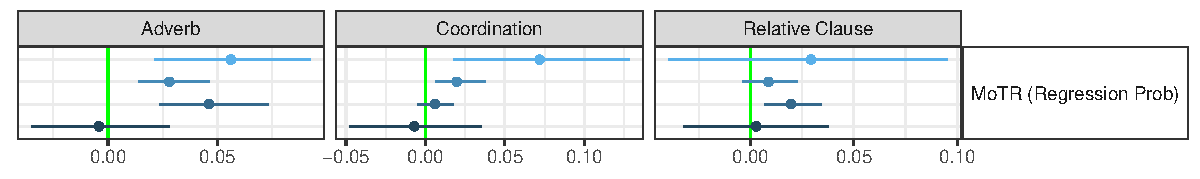
\includegraphics[width=\textwidth]{images/model_estimates_regression160.pdf} 
    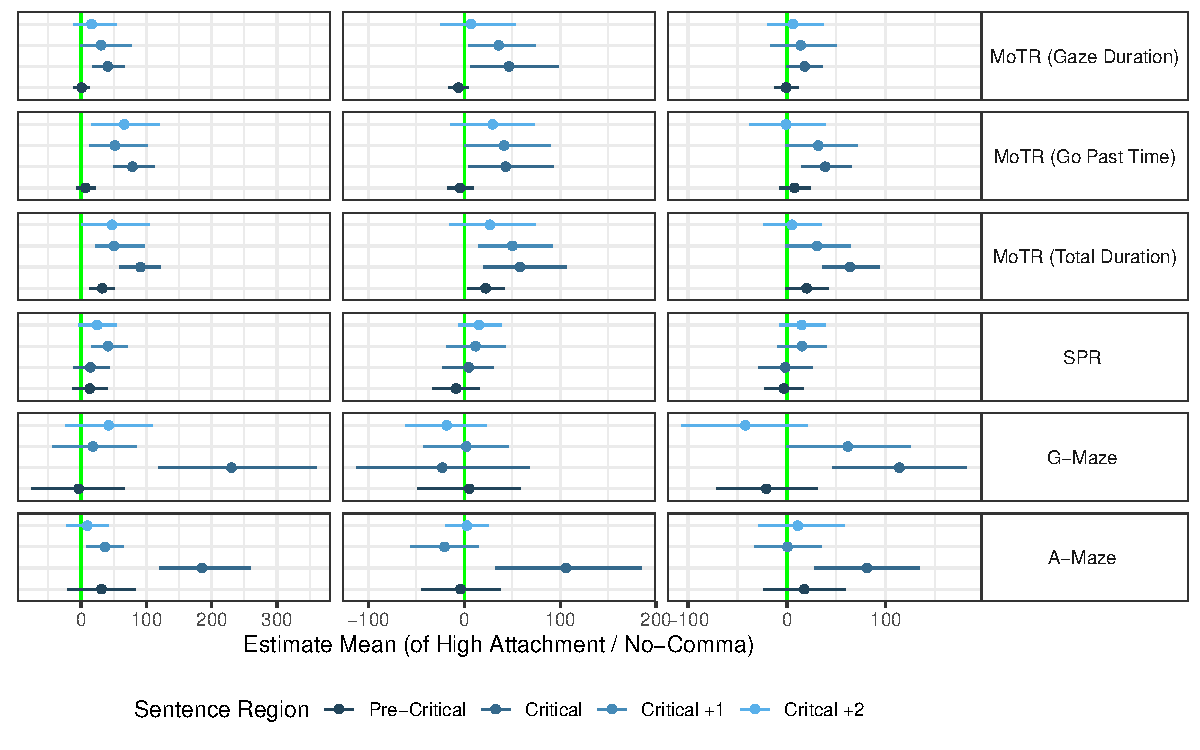
\includegraphics[width=0.98\textwidth]{images/model_estimates160.pdf}
    \vspace{-0.3cm}
    \caption{ \small \textbf{Model Estimates:} Posterior means and 95\% Credible Intervals for the main effect of experimental condition from our Bayesian logistic regression model (top panel) and linear regression models (bottom panels). The $x$-axis scale is in percentages of participants who regress for the top row, and in milliseconds of reading time for all other rows.}
    \label{fig:modeling-results}
    \end{minipage}
\end{figure*}

\begin{figure*}[t]
    \centering
    \begin{minipage}{\textwidth}
    \centering
    \small
    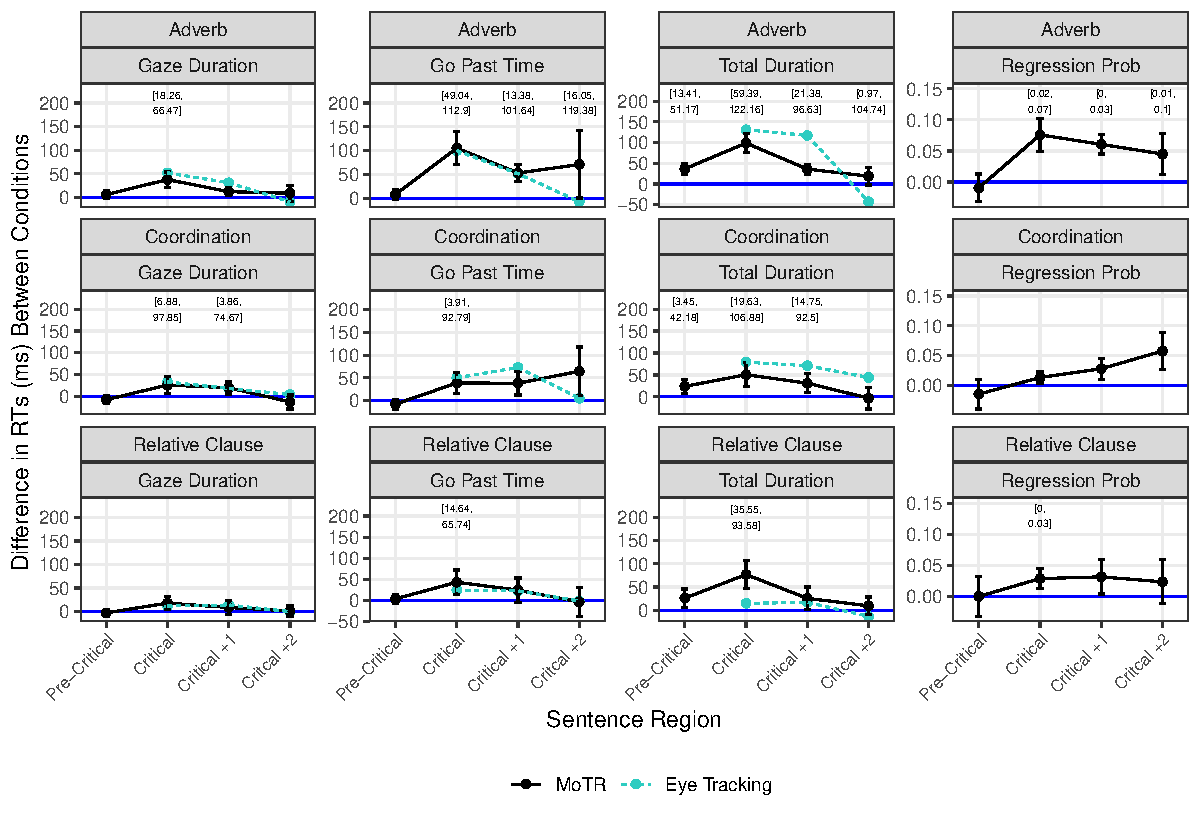
\includegraphics[width=\textwidth]{images/target_results_cris160.pdf}
    \vspace{-0.8cm}
    \caption{ \small \textbf{Main Results:} Points are the by-item mean differences between conditions, where positive values indicate slowdown in \highattach / \nocomma conditions. The right column is the difference in first-pass regression probability, where the $y$-axis indicates the percentage of participants who regress. \motr data is black, eye-tracking reported in \citet{witzel2012maze} is \textcolor{teal}{teal}. Error bars are 95\% confidence intervals of the mean. The text indicates 95\% credible intervals for the effect of condition from our hierachical models when these do not cross zero. The \motr data reveals differences in processing difficulty between conditions and is well-matched to the eye-tracking data.}  
    %Error bars for \motr are 95\% CIs across items. P-values are from mixed-effects regression models fit on the raw \motr data. The \motr data reveals differences in processing difficulty between conditions, and is well-matched to the eye-tracking data. }
    \label{fig:target-results}
    \end{minipage}
\end{figure*}


Focusing first on the Adverb experiment, we found that high attachment leads to longer reading times in the critical region for all metrics: posterior mean $\beta$-weight and 95\% Bayesian credible interval for gaze duration \stats{28}{14}{43}; for go past time \stats{60}{38}{85}; and for total duration \stats{74}{50}{100}. In addition, we find that high attachment leads to longer reading times in the critical+1 region for all metrics as well (for gaze duration: \stats{14}{6}{22}; for go past time \stats{35}{22}{50}; and for total duration: \stats{30}{17}{43}). We find that high attachment leads to increased total duration reading times in the pre-critical condition \stats{28}{14}{43}, indicating that participants are re-reading this region in the high-attachment condition and not in the \lowattach condition. Finally, we find that high attachment leads to greater instances of regressions in the critical region \stats{0.05}{0.03}{0.08}, critical +1 region \stats{0.03}{0.02}{0.05}, and the critical +2 region \stats{0.06}{0.02}{0.09}, which is in line with the relatively larger effects found in go past time over gaze duration, where time spent during the regression is factored into the former but not the latter. 

%we find significant differences between conditions in the critical region for all metrics ($p<0.001$), as well as in the critical +1 and critical +2 regions for go past time ($p<0.001$ and $p<0.05$ respectively). We find a significant effect of condition in the pre-critical region for total duration ($p<0.01$), indicating that participants are making regressions to this region in the high-attachment condition but not in the low-attachment condition. Finally, we find a significant effect of condition on regression probability ($p<0.001$ for the critical and critical + 1 regions; $p<0.05$ for the Critical +2 region), which is in line with the relatively larger effects found in go past time over gaze duration, where time spent during the regression is factored into the former but not the latter.

In the coordination experiment, we found that \nocomma leads to longer reading times in the critical region for all metrics (for gaze duration: \stats{19.43}{1.94}{36.54}; go past time: \stats{23.04}{4.42}{40.84}; and total duration: \stats{35.65}{13.00}{58.11}). We also find that the \nocomma condition leads to longer reading times in the critical +1 region for all metrics as well (for gaze duration: \stats{16.90}{4.64}{28.96}; for go past time: \stats{28.03}{11.26}{44.33}; and for total duration \stats{24.92}{7.98}{41.99}). In line with the adverb experiment, for total duration, we also find longer reading times in the pre-critical region in the \nocomma condition \stats{18.07}{2.93}{33.38}, indicating that participants are making some regressions to this region in the \nocomma condition. Unlike the Adverb experiment, we do not find an effect of condition on regression probability in the critical region. Rather, regression probability in the \nocomma condition increases in the regions following the disambiguating material (for the critical +1 region: \stats{0.02}{0.01}{0.04}; and for the critical +2 region: \stats{0.07}{0.02}{0.13}).

%In the coordination experiment, we find a significant effect of condition on reading times in the critical region for all metrics ($p<0.05$ for gaze duration and go past time; $p<0.001$ for total duration), as well as a significant effect of condition for the crticial +1 region ($p<0.05$ for gaze duration and total duration; $p<0.01$ for go past time). Finally, we find a significant effect in the critical +2 region for go past time ($p<0.05$).  Unlike the Adverb experiment, we do not find an effect of condition on regression probability in the critical region. Rather, regression probability in the no-comma condition increases in the regions following the disambiguating material ($p=0.001$ for critical +1; $p<0.001$ for critical +2).

As with the other experiments, for the relative clause experiment, we found that high attachment leads to reading time slowdowns in the critical region for all metrics (for gaze duration: \stats{14.11}{0.22}{28.21}; for go past time: \stats{25.42}{6.00}{44.85}; and for total duration: \stats{60.39}{33.44}{87.71}). Additionally, we find that high attachment leads to increased regressions in the critical region \stats{0.02}{0.01}{0.03}.
%For the relative clause experiment, we find a significant effect of condition on reading times in the critical region for gaze duration ($p<0.05$) go past time ($p<0.01$) and total duration ($p<0.001$). Additionally, for total duration, we find an effect of condition for the post-critical ($p<0.05$) region. For regression probability, we find an effect of condition for the critical region ($p<0.001$). 

There are three high-level patterns worth commenting on in the data. The first high-level pattern is that the \motr data is able to reveal differences in processing between the conditions, with participants taking longer to read critical regions in \highattach / \nocomma conditions across the different metrics. Second, there is a consistent pattern in the metrics based on the inclusion of regression information, with gaze duration revealing the smallest differences between conditions, go past time revealing medium differences, and total duration revealing the largest differences difference between conditions, on the original millisecond scale. %These patterns validate the basic parallel we have been drawing between the metrics for \motr and eye-tracking. 
They suggest that, in a controlled psycholinguistic setting, \motr can reveal how regressions out of and into sentence regions are implicated in sentence processing.

The final pattern worth mentioning is the tight connection we observe between \motr and eye-tracking data in terms of the magnitudes of the effects. Although, as we saw in Section \ref{sec:exp2}, participants take longer to read words in \motr, on average, the differences in reading times between conditions are well-matched with the differences observed in the eye-tracking data. Indeed, looking at Figure \ref{fig:target-results} for the critical region the eye-tracking data is within the 95\% confidence intervals of the \motr data in 7/9 cases (the exception is total duration in the relative clause and adverb experiments). The major qualitative difference between the two is that: (a) effects at critical regions are larger in \motr for the relative clause experiment, and (b) participants tend to regress more to the post-critical regions in eye-tracking, as evidenced by the higher teal dots in the critical +1 conditions for total duration in the adverb and coordination experiments. This latter difference is likely because regressions are less costly to initiate in eye-tracking, compared with \motr.

\subsubsection{Comparing \motr to Other Web-Based Metrics}

\begin{figure*}[t]
    \centering
    \begin{minipage}{\textwidth}
    \centering
    \small
    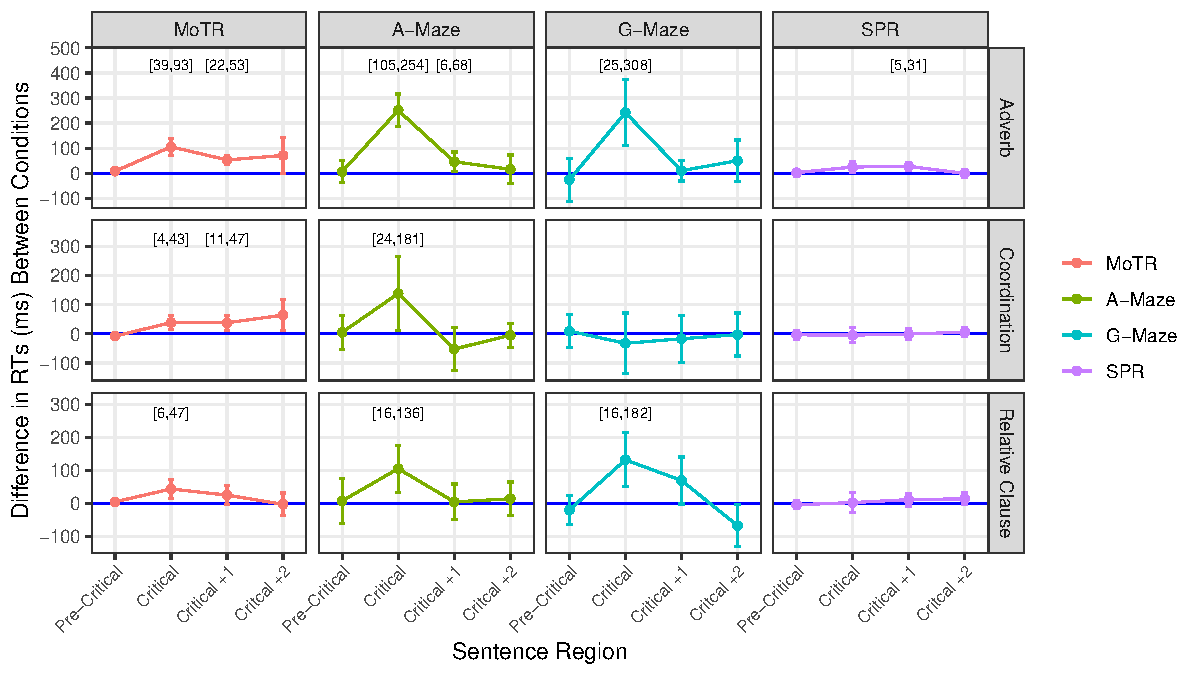
\includegraphics[width=\textwidth]{images/target_comp_cris160.pdf}
    \vspace{-0.8cm}
    \caption{ \small \textbf{Comparison Between Measures:} Comparison between \motr results (go past time) and data from three online incremental processing measurements reported in \cite{boyce2020amaze}. Errors are 95\% CIs across by-item differences; text indicates 95\% credible intervals for the effect of condition from our regression models, when these do not cross zero.}
    \label{fig:target-comp}
    \end{minipage}
\end{figure*}

To get a sense of how \motr compares to other web-based measures of incremental processing, we downloaded the data for web-based A-maze, G-maze, and SPR from \cite{boyce2020amaze} and analyzed it using our methods. The results can be seen in Figure \ref{fig:target-comp}. Unlike \citet{boyce2020amaze}, who report word-by-word averages, we report average differences in reading times for the whole sentence region. We compare the maze and SPR data to \motr go past time. Maze and SPR measure the amount of time that elapses from when the participant first sees a word, to when they progress past it in the sentence, which is essentially what go past time is measuring.

The four metrics differ somewhat in their ability to reveal differences in processing behavior between the conditions. Results for \motr are the same as reported above: We find that the critical condition (i.e., \highattach or \nocomma) leads to slowdowns in all experiments, with slowdowns in the post-critical regions also in the adverb and coordination experiments. Using SPR, we find that high attachment leads to reading time slowdowns only in the adverb experiment critical +1 region \stats{16}{5}{31}. Using G-Maze, we find that high attachment leads to slowdowns in the critical region for the adverb experiment \stats{154}{25}{308} and in the relative clause experiment \stats{96}{16}{182}. Using A-Maze, we find that high attachment leads to slowdowns in the adverb experiment \stats{162}{105}{254} and the relative clause experiment \stats{71}{16}{136}, and that the \nocomma condition leads to slowdowns in the coordination experiment \stats{95}{24}{181}. As far as effect sizes, A-maze and G-maze demonstrate the largest effect sizes, however, we also observe larger variance for these measurements, as indicated by the wider 95\% credible intervals from our models. The tradeoff seems to be that maze will produce larger differences in reading times between conditions, but \motr can pick up on how regressions are implicated in the processing of the phenomena.

%SPR finds an effect of condition on processing time for one experiment (adverb; critical +1 where $p<0.01$). G-maze finds differences in critical regions for two experiments (Adverb, where $p<0.001$; and Relative Clause where $p<0.01$). Like \motr, A-maze finds an effect in all three experiments on the critical region (Adverb $p<0.001$; Coordination $p<0.05$ and Relative Clause $p<0.05$). As far as effect sizes, A-maze and G-maze demonstrate the largest effect sizes, however we also observe larger variance for these measurements, as indicated by the wider 95\% confidence intervals in Figure \ref{fig:target-comp}. The tradeoff seems to be that maze will produce larger differences in reading times between conditions, but \motr can pick up on how regressions are implicated in the processing of the phenomena.

\subsection{Discussion}

%To demonstrate the potential utility of a \motr experiment, we briefly discuss how it reveals processing differences between our three sub-experiments, something which is not evident in the maze data, nor obvious in the eye-tracking data. These differences have to do with the role of regressions during processing, specifically, when a regression is initiated. In the relative clause experiment, we observe that the difference in regression rate between the conditions falls only in the critical region itself. That is, participants are more likely to regress on the reflexive pronoun that forces high-attachment, but not subsequently in the sentence. For the adverb experiment, we observe a similar difference in regression rate in the critical region, however this difference is sustained in both post-critical regions as well. This can be observed both in the higher difference in regression rates for these regions, as well as in the larger difference in go past time RTs observed in this experiment. In the coordination experiment, the pattern of results is quite different. Here, we observe no difference in regression rate between conditions in the critical region. This indicates that, although participants slow down at the disambiguating verb, they are not credibly more likely to initiate a regression in the no-comma condition. 

%At a high level, these patterns are consistent with two different processing strategies---an immediate regression strategy that is used during the processing of adverbs and relative clauses, and a sentence-final regression strategy that is used when processing NP/Z gardenpaths. 
%At a high level, these patterns are consistent with two different strategies, one that relies on regressions to facilitate reanalysis of the sentence, and one where reanalysis occurs without the aid of regressions. We would like to stress, however, that further experimental validation of these results should be conducted before strong theoretical conclusions are drawn.

To demonstrate the potential utility of a \motr experiment, we briefly discuss how it reveals processing differences between our three sub-experiments, something which is not evident in the maze data, nor obvious in the eye-tracking data. These differences have to do with the role of regressions during processing, specifically, when a regression is initiated. In the relative clause experiment, we observe that the difference in regression rate between the conditions falls only in the critical region itself. That is, participants are more likely to regress on the reflexive pronoun that forces high-attachment, but not subsequently in the sentence. For the adverb experiment, we observe a similar difference in regression rate in the critical region, however, this difference is sustained in both post-critical regions as well. This can be observed both in the higher difference in regression rates for these regions, as well as in the larger difference in go past time and total duration RTs observed in the critical, critical +1, and critical +2 regions for this experiment. In the coordination experiment, the pattern of results is quite different. Here, we observe no difference in regression rate between conditions in the critical region, but a steady increase of regression rate difference in the \nocomma condition for both post-critical regions. This indicates that, although participants slow down at the disambiguating verb, they save their regressions for the end of the sentence. 

At a high level, these patterns are consistent with two different processing strategies---an immediate regression strategy that is used during the processing of adverbs and relative clauses, and a sentence-final regression strategy that is used when processing NP/Z gardenpaths. We would like to stress, however, that further experimental validation of these results should be conducted before strong theoretical conclusions are drawn.

Turning back to the main question posed at the beginning of this section, we find that \motr can, indeed, measure well-studied language processing patterns in English. Across experiments and metrics, we observe a robust slowdown for processing high-attachment sentences, which is consistent with prior work in this area. Thus, the results from this experiment demonstrate that \motr can be used to reveal processing behavior in a targeted psycholinguistic setting.


\section{General Discussion}


We begin our discussion by turning back to the three considerations mentioned in the introduction---precision, naturalness, and cost. Starting, first, with cost, it’s evident the \motr is as cheap to run as the cheapest current alternatives, maze and SPR. Because it runs in the browser, it is possible to use the paradigm for studies that recruit large numbers of participants over the Internet. Although we did not test this directly in our experiments, it’s also possible to run \motr experiments locally in the browser, meaning that \motr can be used wherever computers are available, such as in labs not equipped with eye-trackers and, potentially, in fieldwork.

Turning to naturalness, we argue that this aspect of \motr sets it apart from the other web-based measures, SPR and maze. In both traditional (moving window) SPR and maze participants are both unable to skip words and regress to previous words, making these techniques much more constrained than eye-tracking and potentially less ecologically valid as measurements of reading behavior. While making saccades in a \motr trial requires coordinating hand and eye movement, our data suggests this does not inhibit participants from engaging in more naturalistic behavior that involves more than just a linear pass over the text. For example, in the Provo experiment, we find that, on average, participants make regressions in 4\% of words and skip about 45\% of words, compared to a regression rate of 15\% and a skip rate of 44\% in eye-tracking. While regression rates are certainly lower in \motr, it’s also clear that participants take advantage of the paradigm to make flexible scanpaths through the materials.

Turning to the question of precision, it's clear that eye-tracking still offers the most precise behavior measurements for psycholinguistic reading research. However, \motr may have an advantage over eye-tracking when it comes to preview effects. Because it is difficult in eye-tracking studies to control the extent of parafoveal processing (unless in gaze contingency or boundary paradigms), the extent to which preview effects influence observed behavior is difficult to determine when it comes to eye-tracking. Because upcoming words are occluded in \motr (as well as in maze and SPR), this potential preview effect can be ruled out therefore excluding any effects of parafoveal processing that were not intended by the researcher or the experimental design. Unlike in maze and SPR, however, upcoming words in \motr are not fully occluded (they are simply blurred) and the participant can partially reveal some upcoming material with the gradual transition effect of the spotlight. That being said, a \motr experiment does enable the experimenter to know for certainty what was in focus and what was blurred and thus unreadable at any given point in time.

As far as precision, how does \motr compare against SPR and maze? While SPR does not pick up on any of the differences between conditions in Experiment 1, both \motr and A-maze show robust slowdowns in the \highattach and \nocomma conditions. A-maze recovers larger magnitudes in processing times between conditions and is potentially more incremental insofar as most of its effects are solely on the critical region. In \motr, some of the effects are in post-critical regions—--for example, for gaze duration in the coordination experiment. However, \motr still picks up robust differences between conditions and, to its advantage, its effect sizes are more in line with those observed in the eye-tracking data. We believe that \motr and maze can offer useful complements to each other.  In cases where only incremental processing slowdowns are necessary for evaluating theoretical claims, then maze may be the more revealing experimental tool. However, in cases where information about regression and skipping as well as processing slowdown are important, then \motr may be the better choice.


We designed the experiments in this paper to offer a balance between the type of experiments that are traditionally used to assess psycholinguistic theories, including both targeted psycholinguistic minimal pairs and naturalistic materials. Furthermore, we have done so with materials for which previously collected maze, SPR, and eye-tracking data are already available. There is one major gap in our assessment, however, and this is that our studies were collected entirely in English. Testing \motr on a more diverse range of languages is an obvious next step in order to fully validate this new measurement.

% Future directions: Mention that we have an anecdote with someone who has a language impairment and that this could be a future direction. Say it was feedback from online participants.
% Could also be useful for language education. Helping children learn to read.


\section*{Acknowledgements}

EGW was supported by an ETH Postdoctoral Fellowship. LAJ would like to acknowledge funding from the Swiss National Science Foundation under grant 100015L 212276/1 (MeRID). 

\bibliographystyle{apalike}
\bibliography{everything}




\end{document}